\section{Low Energy Excess Overview and Motivation}
\subsection{Introduction}
This chapter will describe the MicroBooNE analysis centered around searching for the observed low energy excess reported by its predecessor experiment, MiniBooNE. A historical background motivating this analysis is provided (the LSND experiment which first observed an excess of $\overline{\nu}_e$ in a $\overline{\nu}_\mu$ beam). Then, a description of the MiniBooNE experiment (detector and analysis) is provided. As will be shown, MiniBooNE observed an unexplained excess of electron-like events in a primarily $\nu_\mu$ beam in the neutrino energy region between 200 to 475 MeV, and MicroBooNE will search for that same excess in the same neutrino beam-line, but with a different detector technology.\\

With historical context in perspective, this chapter then discusses the analysis to determine the sensitivity of the MicroBooNE detector to measure the same signal as MiniBooNE, with some assumptions about that signal (that the excess originates from an excess of beam-induced $\nu_e$ interactions). This discussion covers the signal modeling based on the MiniBooNE published data releases. The event selection and background mitigation techniques in MicroBooNE are described, and ultimately the expected sensitivity to measure such a signal is calculated.

\subsection{LSND Observation}
%Brief discussion of the LSND experiment and how they saw an excess of antinue in the antinumu beam with L/E that didn't fit in with any measured mixing angles and delta m2 in 3 neutrino model.

In 2001, the Liquid Scintillator Neutrino Detector (LSND) collaboration published an observation of excess events consistent with $\overline{\nu}_e$ interactions above the expected background in a $\overline{\nu}_\mu$ beam at the Los Alamos Neutron Science Center \cite{LSNDPaper}. Given the $\frac{L}{E}$ ($\approx$ $\frac{30 m}{40 MeV}$) for this measurement, the excess disagreed with previous measurements of neutrino mixing angles and $\Delta m^2$ values in the three neutrino model. The LSND excess corresponded to a $\Delta m^2$ of approximately 1 $eV^2$, orders of magnitude higher than previously measured values of $\Delta m_{12}^2$ and $\Delta m_{23}^2$. One explanation for this drastically different $\Delta m^2$ value is the existence of potential additional ``sterile'' neutrino states, which must not interact weakly given the Z- boson decay width constrains the number of weakly interacting neutrino states to three.\\

To test the LSND result, the MiniBooNE experiment was designed. It would measure $\nu_e$ interactions in a primarily $\nu_\mu$ beam, with a similar $\frac{L}{E}$ ($\approx$ $\frac{500m}{700 MeV}$).


\subsection{The MiniBooNE Experiment}

\subsubsection{The MiniBooNE Detector and Monte Carlo Simulation}

%Description of the detector, a schematic figure, description of cherenkov rings, the location of the detector in the BNB. Discussion of how they use NUANCE, mention they use identical beam simulation and reweighting (reweighting should be covered in the beam chapter).


The MiniBooNE detector \cite{MBDetectorPaper} consists of a spherical tank located 541 meters downstream of the BNB neutrino production target, with diameter of 12.2 meters filled with 818 tons of mineral oil underneath at least 3 meters of earth overburden as shown in Figure \ref{MB_detector_fig}. As seen in the figure, there exists an opaque barrier separating a veto region and a signal region. The walls of the signal region are painted black to reduce re-scattering of light and are instrumented with 1280 8-inch photomultiplier tubes (PMTs), most of which were reused from the LSND experiment. In the signal region, the photocathode coverage is 11.8\%. This region is intended to identify beam neutrino interactions happening within it; the PMTs face radially inwards. The veto region is 35 cm thick and is instrumented with 240 PMTs which face tangent to the detector radius and its purpose is to reject backgrounds coming from outside of the detector (cosmics, which have a rate at the detector location of about 10 kHz). The inner surface of the veto region is coated in a reflective paint. The efficiency for rejecting cosmic ray muons with the outer veto region was measured to be 99.99\%.\\

\begin{figure}[ht!]
\centering
	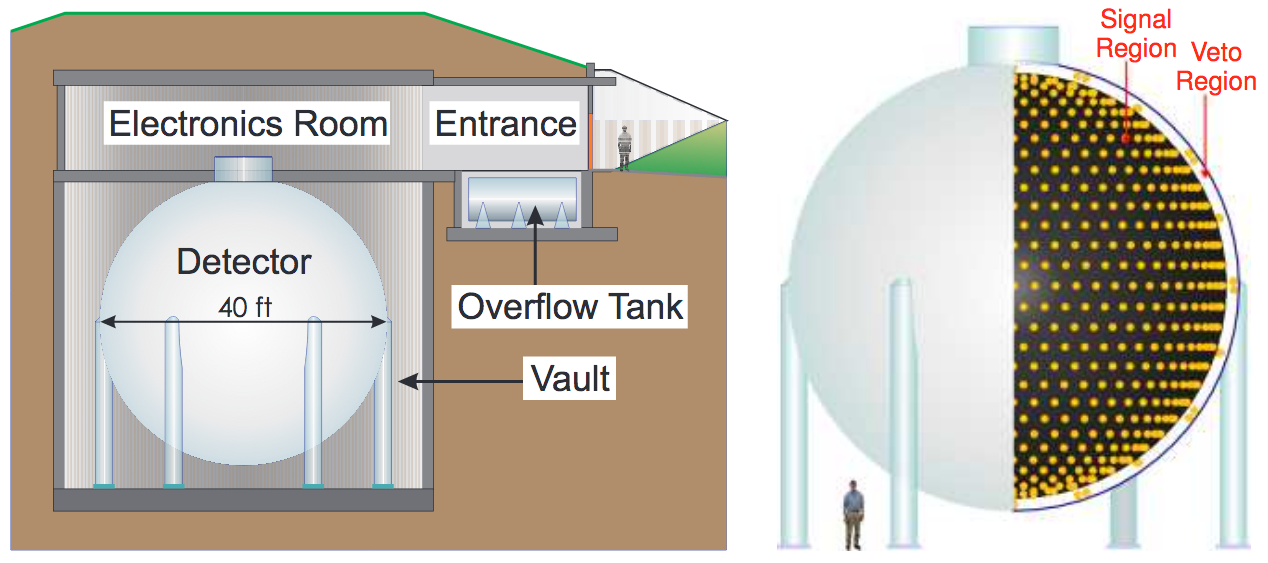
\includegraphics[width=0.9\textwidth]{Figures/MB_detectorpaper_fig.png} \\
\caption{\textit{The MiniBooNE detector enclosure (left) and a cut-away drawing (right) of the detector showing the distribution of PMT's in the signal and veto regions.}}\label{MB_detector_fig}
\end{figure}

The detection method of the MiniBooNE experiment is based primarily on Cherenkov light. The mineral oil within the signal region acts as the neutrino target material. The majority of final state particles exiting neutrino interactions at neutrino energies from the BNB are produced above Cherenkov threshold. These particles produce Cherenkov light which is detected by the PMTs lining the signal region of the detector. Reconstructing the pattern this light projects onto the walls of the signal region allows for some particle identification abilities.\\

The detector is calibrated with a series of \textit{in situ} measurements, primarily with cosmic ray muons. Cosmic ray muons stopping within the detector along with an external muon hodoscope provide for angular resolution measurements. Additionally, muons which stop and produce decay electrons that have a known energy endpoint of around 50 MeV provide an energy calibration source at low energies, while through-going muons provide calibration information at higher energies. Also, tagged $\pi^0$ particles which decay into two photons have a known mass of around 135 MeV and therefore provide energy calibration information in that region.\\

For more details about the MiniBooNE detector, see Appendix \ref{MINIBOONE_APPENDIX_DETECTOR}.

\subsubsection{MiniBooNE Event Selection}
% Brief description of their event selection cuts, mention that the energy definition they use is CCQE and they're looking specifically for CCQE topologies, description of what CCQE means. Figure of their results indicating the excess in neutrino mode. 

Different final state particles exiting a neutrino interaction in the MiniBooNE signal volume create different patterns of Cherenkov light read out by the PMTs. Figure \ref{georgia_cherenkov_cartoon_fig} \cite{GeorgiaThesis} shows how these patterns differ for different common kinds of final state particles (muons, electrons/photons, and neutral pion decays). A muon track produces a crisp, filled-in ring of Cherenkov light, while an electron or photon produces a more fuzzy, hollow ring. A neutral pion decay will result in two photons. By reconstructing these patterns in the PMT data read out from a triggered event in MiniBooNE, the flavor and energy of the interacting neutrino can be determined. With this kind of detection technique it is important to note that a single photon signal is indistinguishable from that of a single electron signal, an important ingredient to the ultimate ambiguity of the observed low energy excess in MiniBooNE.\\

\begin{figure}[ht!]
\centering
	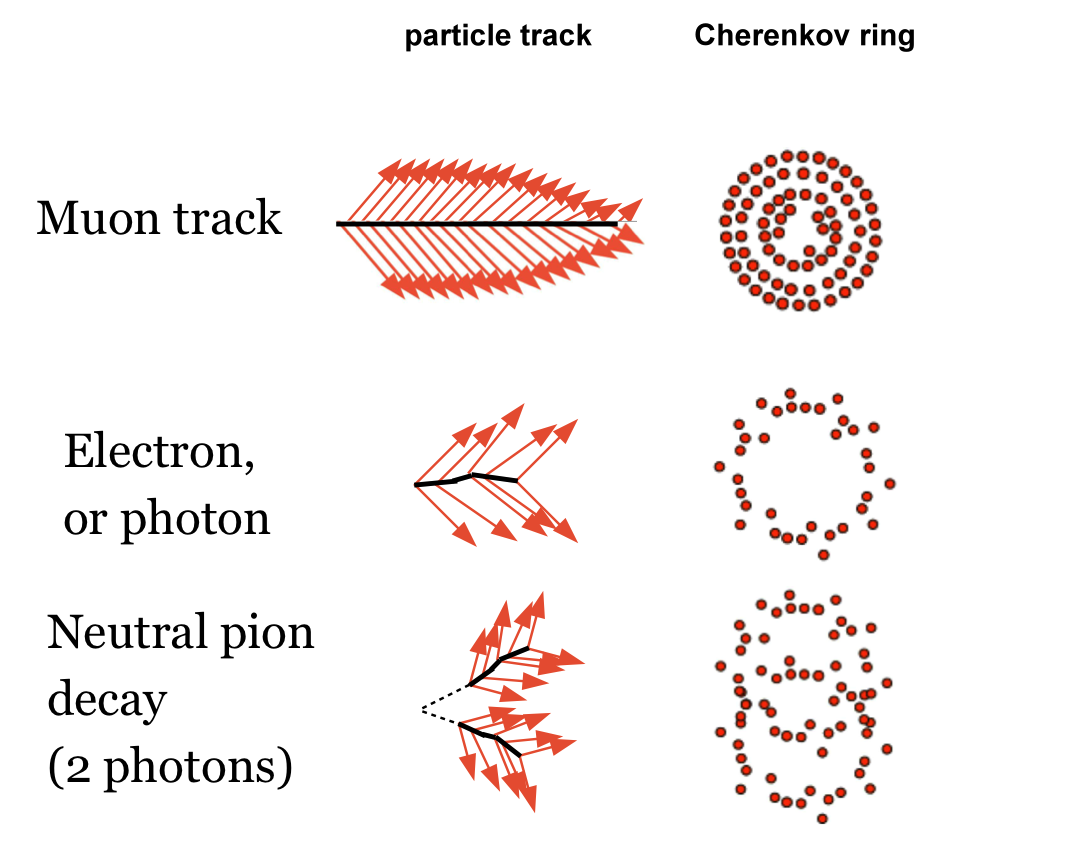
\includegraphics[width=0.9\textwidth]{Figures/georgia_cherenkov_cartoon.png} \\
\caption{\textit{A schematic of the pattern Cherenkov light from different particles would make projected onto the inner walls of the MiniBooNE detector. Top is a muon track (a filled-in ring), middle is an electron (a fuzzy ring), bottom is a photon that pair-produces and creates two fuzzy rings.}}\label{georgia_cherenkov_cartoon_fig}
\end{figure}

The topology of interest in the MiniBooNE oscillation search is that of charged-current quasi-elastic (CCQE) interactions, shown in Figure \ref{georgia_ccqe_feynman_fig}. This interaction channel is the dominant one in the neutrino energy range of the BNB, around 1 GeV $E_\nu$. In a $\nu_l$ CCQE interaction (where $l$ is the neutrino flavor), a lepton of flavor $l$ is produced, along with a proton. The single outgoing lepton is the characteristic event signature for which MiniBooNE searches.\\


\begin{figure}[ht!]
\centering
	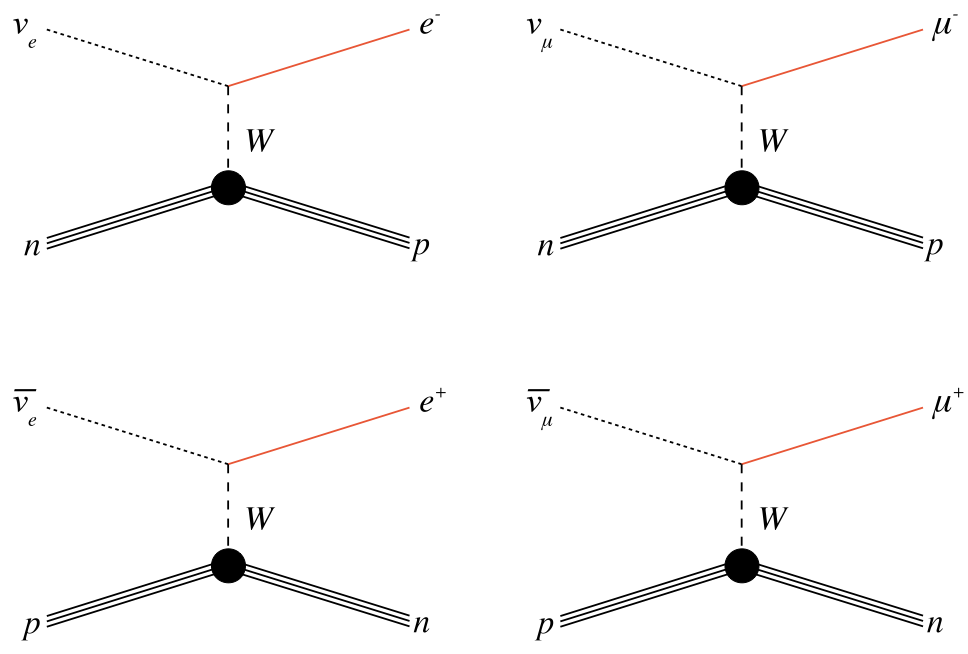
\includegraphics[width=0.9\textwidth]{Figures/georgia_ccqe_feynman.png} \\
\caption{\textit{Feynman diagrams of the charged-current quasi-elastic (CCQE) interaction channel for $\nu_e$, $\nu_\mu$, $\overline{\nu_\mu}$, and $\overline{\nu_e}$ (clockwise from the top left). $\nu_e$ CCQE is the signal channel for the MiniBooNE oscillation analysis.}}\label{georgia_ccqe_feynman_fig}
\end{figure}


In order to select $\nu_e^{CCQE}$ events, cuts are placed to mitigate backgrounds. The most powerful rejection comes from requiring the events occur within the beam timing window. The beam arrives at the detector at a rate of 5 Hz, and each spill lasts 1.6 $\mu s$ and is composed of approximately 80 buckets separated by 19 $ns$. Given the time scale with which MiniBooNE measures the light from interactions, cuts on event timing alone reduces non-beam backgrounds to $\sim10^{-3}$. Two additional cuts are used that require there be more activity within the signal volume than the outer veto volume, a signature characteristic of beam related neutrino events. These pre-cuts achieve more than a 99.99\% rejection of beam unrelated backgrounds. The efficiency to select $\nu_e^{CCQE}$ events in MiniBooNE is on the order of 25\% \cite{JocelynMonroeThesis}.\\

In order to reconstruct events, MiniBooNE uses a maximum likelihood fitting algorithm leveraging properties of charged particle tracks inferred from measured charges and times on the PMTs. The likelihoods to different event hypothesis are used to classify each event as a signal $\nu_e$ CCQE event, or as a background process like $\nu_\mu$ CCQE and NC $\pi^0$ production. Note that MiniBooNE cannot differentiate between a $\mu^+$ and a $\mu^-$, or $e^+$ and $e^-$ so discrimination between neutrino and antineutrino on an event-by-event basis is impossible.\\

Assuming CCQE kinematics, the incident neutrino energy is reconstructed with knowledge of the outgoing lepton energy ($E_l$) and scattering angle ($\theta_l$). In MiniBooNE specifically, the struck nucleon is assumed to be at rest, so the incident neutrino energy $E_\nu^{CCQE}$ is given by:
\begin{equation}\label{MB_CCQE_formula}
E_\nu^{CCQE} = \frac{2m_nE_l+m_p^2-m_n^2-m_l^2}{2(m_n-E_l+\cos\theta_l\sqrt{E_l^2-m_l^2})}
\end{equation}
where $m_n$, $m_p$, $m_l$ are the masses of the neutron, proton, and lepton respectively, and $\theta_l$ is the scattering angle of the outgoing lepton with respect to the (known) beam neutrino direction.\\

\subsubsection{MiniBooNE Results}
%http://www-boone.fnal.gov/slides-talks/conf-talk/shaevitz/shaevitz-lownu.pdf
%http://www-boone.fnal.gov/slides-talks/conf-talk/zdjurcic/Djurcic_MiniBooNE_NuFact2010.pdf
With the described reconstruction methods and energy definition, the MiniBooNE published results \cite{MBLEEPaper} for the $\nu_e$ appearance search in neutrino mode running are shown in Figure \ref{MB_published_stackedhisto_fig}. Note that besides the irreducible intrinsic $\nu_e$ backgrounds, the dominant background in the excess region is $\pi^0$ MID (red). In a $\pi^0$ MID event event, a $\pi^0$ is created in the neutrino interaction and its subsequent immediate decay into two photons mimics a the $\nu_e$ CCQE signature (either one photon escapes, or rings overlap). Another important background is $\Delta\rightarrow N\gamma$ (brown). Recall that both of these backgrounds arise from MiniBooNE's inability to distinguish electrons from photons, an important ambiguity which will be discussed in more detail in the following sections.\\


\begin{figure}[ht!]
\centering
	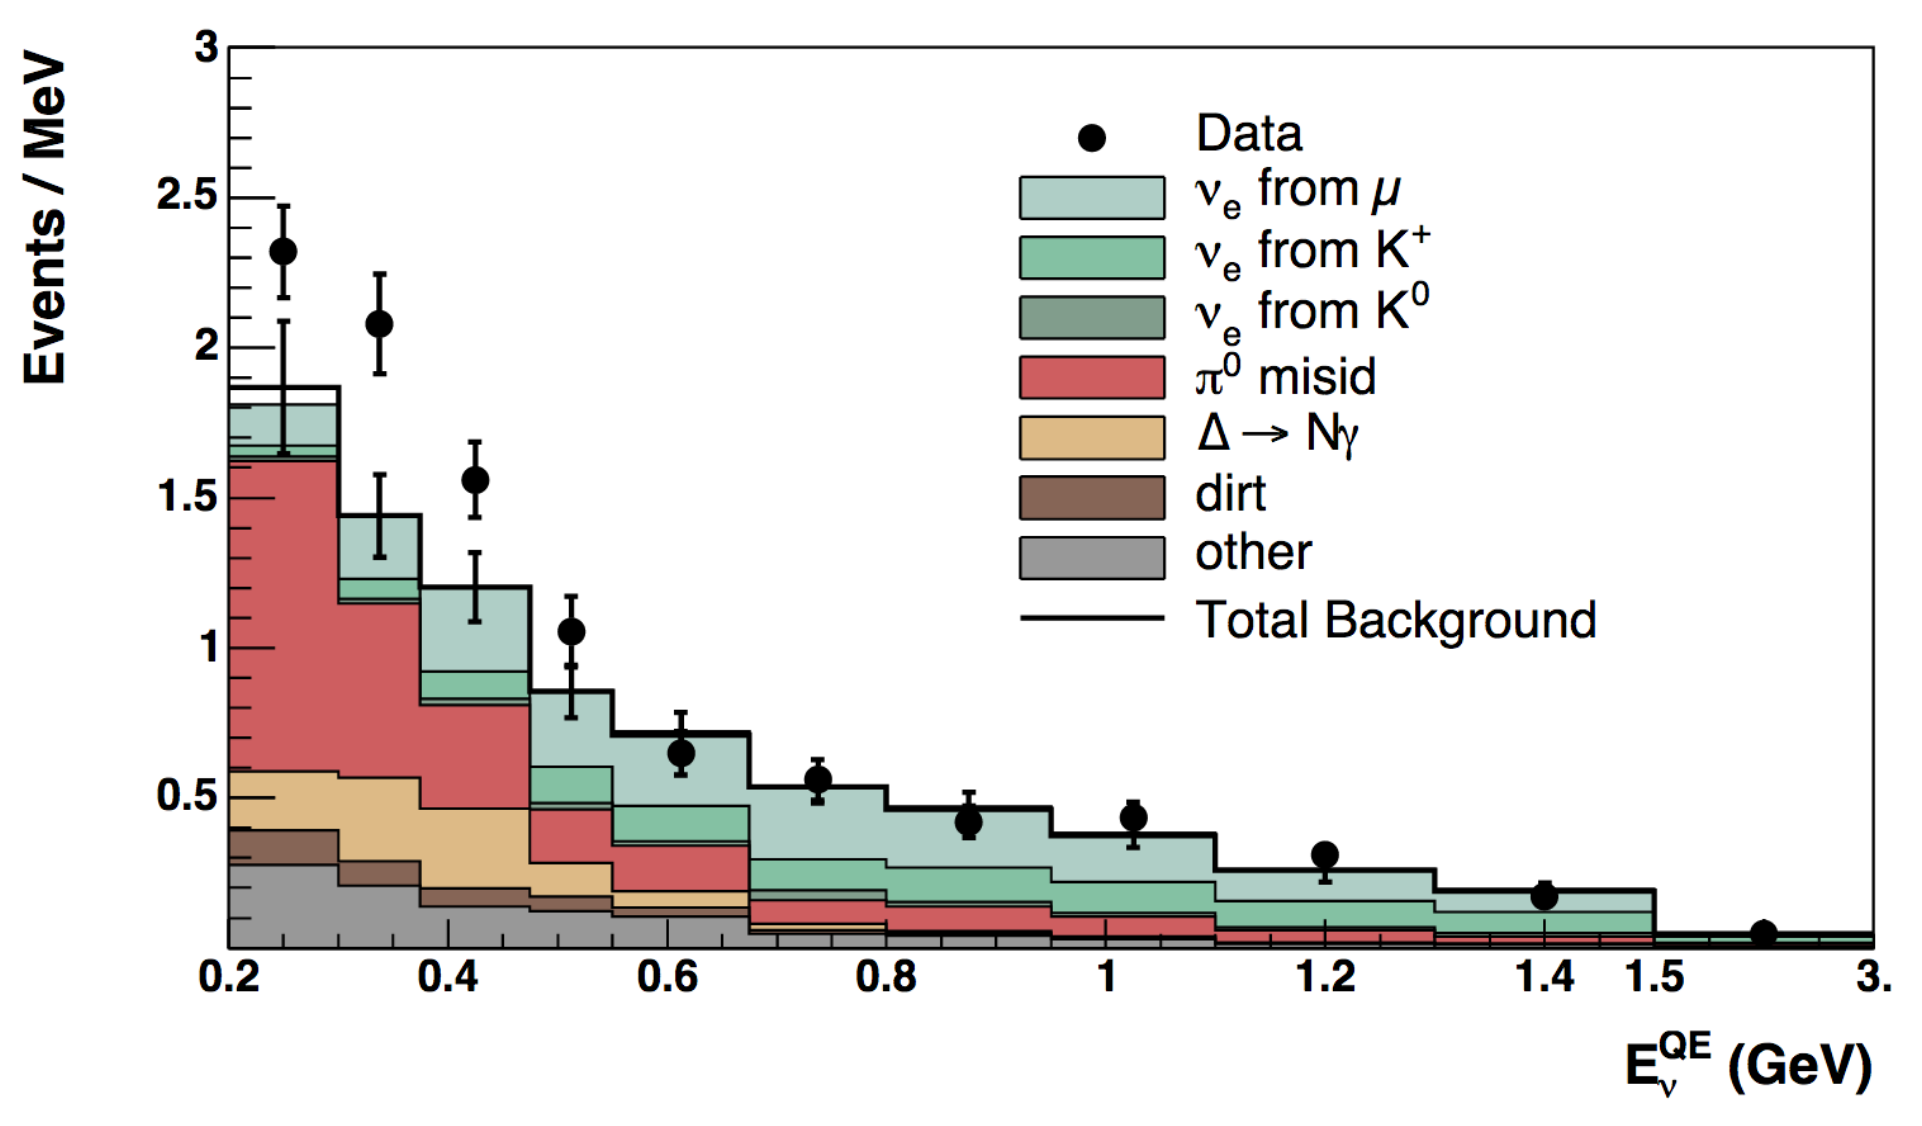
\includegraphics[width=0.9\textwidth]{Figures/MB_published_stackedhisto.png} \\
\caption{\textit{The $E_\nu^{QE}$ distribution for MiniBooNE data (points with statistical errors) and and backgrounds (histogram with systematic errors).}}\label{MB_published_stackedhisto_fig}
\end{figure}


As shown in Figure \ref{MB_published_stackedhisto_fig}, in the energy region $E_\nu^{QE} > 475$ MeV there is good agreement between data and background prediction, making a two neutrino fit inconsistent with the LSND results at the 98\% confidence level assuming CP conservation. Meanwhile, below $E_\nu^{CCQE}$ of 475 MeV there is a statistically significant (6$\sigma$, reduced to 3$\sigma$ after systematics) excess. The excess of 129 $\pm$ 43 events (stat+syst) is consistent in magnitude with the LSND oscillations.\\


In a later separate antineutrino run (in which the BNB horn current is switched to produce a primarily $\overline{\nu}_\mu$ beam), an excess was observed in the energy region $E_\nu^{QE} > 475$ MeV that was consistent with an LSND-type two neutrino oscillation over the null oscillation hypothesis at the 91\% confidence level. In the lower energy region $E_\nu^{QE} < 475$ MeV, an excess of 38.6 $\pm$ 18.5 events was observed. In a fit to the full energy range $E_\nu^{QE} > 200$ MeV, the excess was consistent with an LSND-type two neutrino oscillation over the null oscillation hypothesis at the 98\% confidence level.\\


\subsubsection{Proposed Low Energy Excess Sources}

% The LEE could either be electron like or photon like, MiniBooNE couldn't tell. Mention of theories like sterile neutrinos though no models seem to fit very well (3+1 or 3+2 with possible CP violation), single photon background misestimations or unexpected backgrounds, neutrino decay, lorentz violation etc etc. 
Shown in Figure \ref{MB_published_excess_fits_fig} is the MiniBooNE neutrino mode excess (data - expected background) with oscillation fits with parameters constrained to be in the LSND allowed region. The parameters in the LSND allowed region are ruled out at the 95\% confidence level if the data are fit with $E_\nu^{CCQE}>$ 475 MeV. \\

\begin{figure}[ht!]
\centering
	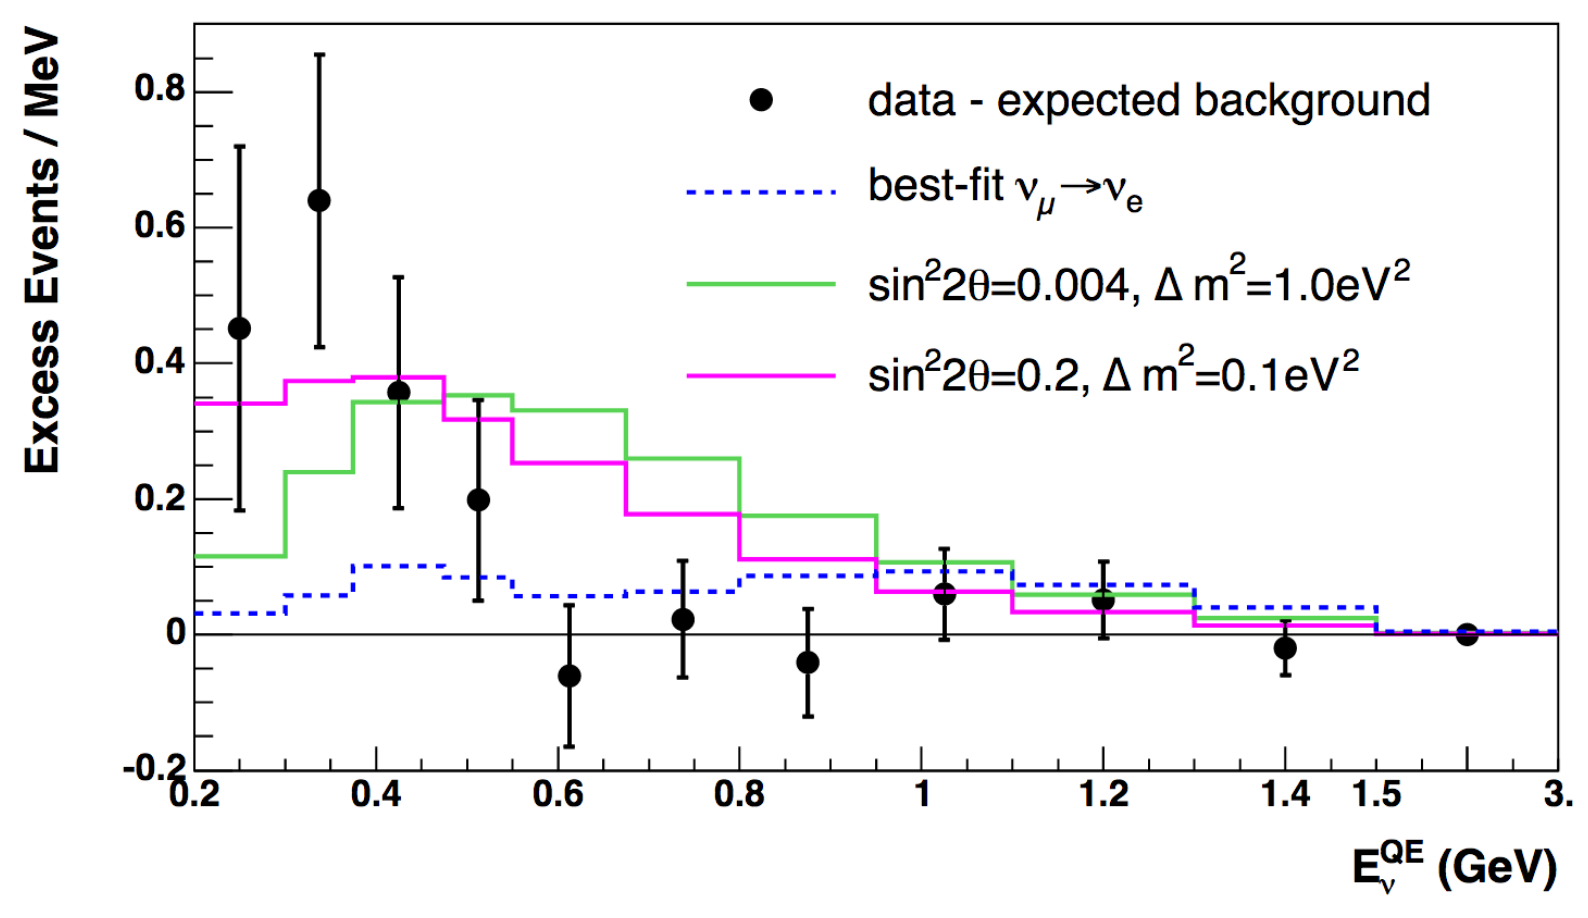
\includegraphics[width=0.9\textwidth]{Figures/MB_published_excess_fits.png} \\
\caption{\textit{The MiniBooNE event excess as a function of $E_\nu^{QE}$. Also shown are the expectations from the best oscillation fit and from neutrino oscillation parameters in the LSND allowed region. The error bars include both statistical and systematic errors.}}\label{MB_published_excess_fits_fig}
\end{figure}

Given MiniBooNE's inability to distinguish electrons from photons, the origin of this excess is either a mis-estimation of one of the backgrounds, or some sort of new physics. The former is unlikely the case because MiniBooNE makes many \textit{in situ} measurements that allow for the constraining of these backgrounds. The neutral current induced backgrounds (NC $\pi^0$, $\Delta\rightarrow N\gamma$, and dirt) are constrained by such measurements. Measurements constraining these backgrounds are described in more detail in the following paragraphs.\\

The NC $\pi^0$ rate in MiniBooNE is measured by selecting events with reconstructed mass near the $\pi^0$ mass. This obtains a $>90$\% pure sample of NC $\pi^0$ interactions which is compared to simulation to obtain a correction function in order to bring the simulated distribution in agreement with data. This same correction function is applied to NC $\pi^0$ events that are backgrounds in the $\nu_e$ appearance analysis. This correction function increases the NC $\pi^0$ background by less than 13\% for $E_\nu^{CCQE}$ $<$ 400 MeV and decreases the background by as much as 20\% above this neutrino energy region. Including this correction factor, the uncertainty on the overall NC $\pi^0$ backgrounds is 7\%. Note that a correction factor of 2.0 would be required to explain the origin of the excess as originating from a mis-estimated NC $\pi^0$ background \cite{GeorgiaThesis}.\\

The excess is unlikely caused by a mis-estimation of the $\Delta\rightarrow N\gamma$ backgrounds because they are additionally constrained by the NC $\pi^0$ measurement through the relative rate of resonant production times a branching fraction of (0.56$\pm$0.04)\%. With this measurement, the uncertainty on the $\Delta\rightarrow N\gamma$ backgrounds is 12\%. Note that a (very large) correction factor of 2.7 would be required to explain the origin of the excess as originating from a mis-estimated $\Delta \rightarrow N\gamma$ background.\\

The excess is unlikely caused by a mis-estimation of the dirt backgrounds because a direct measurement is made by selecting a separate event sample which are likely dirt events and comparing data to simulation. These events are reconstructed close to the detector boundaries with direction pointed generally inwards. In neutrino mode, a dirt background normalization correction factor was computed to be 0.7 $\pm$ 0.1 (with simulation over-predicting the dirt rate normalization). Given the power of the event selection cuts designed to mitigate dirt backgrounds, the relevance of this relatively large correction factor is minimal.\\

The charged current induced backgrounds (intrinsic $\nu_e^{CCQE}$) are reduced with \textit{in situ} measurements of $\nu_\mu$CCQE interactions. A data to simulation comparison of measured $\nu_\mu$CCQE interactions allows for the retuning of underlying flux and cross section parameters in order to bring simulated distributions in agreement with data. These parameters are the same as those used to predict the $\nu_e^{CCQE}$ rate and shape. In addition, a measurement of the highest energy $\nu_\mu$CCQE interactions allows for the further constraint of $\nu_e^{CCQE}$ from kaon decay backgrounds, which is discussed in more detail in a later section of this thesis.\\

Given the likelihood that the excess is not caused by misidentified backgrounds, several new-physics interpretations have been proposed in attempt to explain the excess, including sterile neutrino oscillations (with one, two, or more sterile neutrinos), and new interactions both within and outside of the standard model (CPT violation, quantum decoherence, sterile neutrino decay, etc). A summary of these interpretations can be found in \cite{MBLEESourcesOverview}. A commonality between all interpretations is that their interactions pass the MiniBooNE event selection cuts; that is, they have one electron or one photon exiting the interaction vertex.

\subsection{MicroBooNE In The Context of the Low Energy Excess}
% Discussion of how as a LArTPC MicroBooNE has electron/photon separation. Showing the scaled signal plot from the TDR. Mention that this scaled signal is oversimplified so that's why this thesis describes a more rigorous sensitivity study with simulation in MicroBooNE.

%http://microboone-docdb.fnal.gov:8080/cgi-bin/RetrieveFile?docid=3528&filename=low-E-excess-note.pdf&version=2
Given the proposed explanations for the origin of the measured MiniBooNE low energy excess in neutrino mode all predict either a single electron or single photon produced at the neutrino interaction vertex, and that MiniBooNE cannot discriminate between single electrons or photons, the MicroBooNE experiment was proposed. This detector (described in detail in Section \ref{UBDetectorSection}) is a liquid argon time projection chamber, a relatively new detector technology which allows for the discrimination between single electrons and photons. MicroBooNE runs in the same beam line (BNB) in neutrino mode and is physically located close to MiniBooNE. Therefore, MicroBooNE should be able to elucidate the MiniBooNE low energy excess ambiguity, first by seeing if an excess exists and then determining if the excess is related to an excess of photon events or electron events.\\

The electron/photon discrimination power of a LArTPC is based on the energy deposition at the start of electron and photon showers (photons will pair produce and in general have twice the ionization as a single electron). Shown in Figure \ref{UB_TDR_egammadedx_fig} is the energy loss per unit length along the first 2.4 cm of simulated single electron showers (red) and single photon showers (black) in terms of minimally ionizing particle (MIP) energy in liquid argon (about 2.1 MeV/cm). Leveraging the dE/dx difference between electrons and photons, and additionally the presence of a several centimeter (on average) gap between a photon's creation point and its pair production, MicroBooNE has very powerful electron/photon separation power whereas MiniBooNE has none.\\

\begin{figure}[ht!]
\centering
	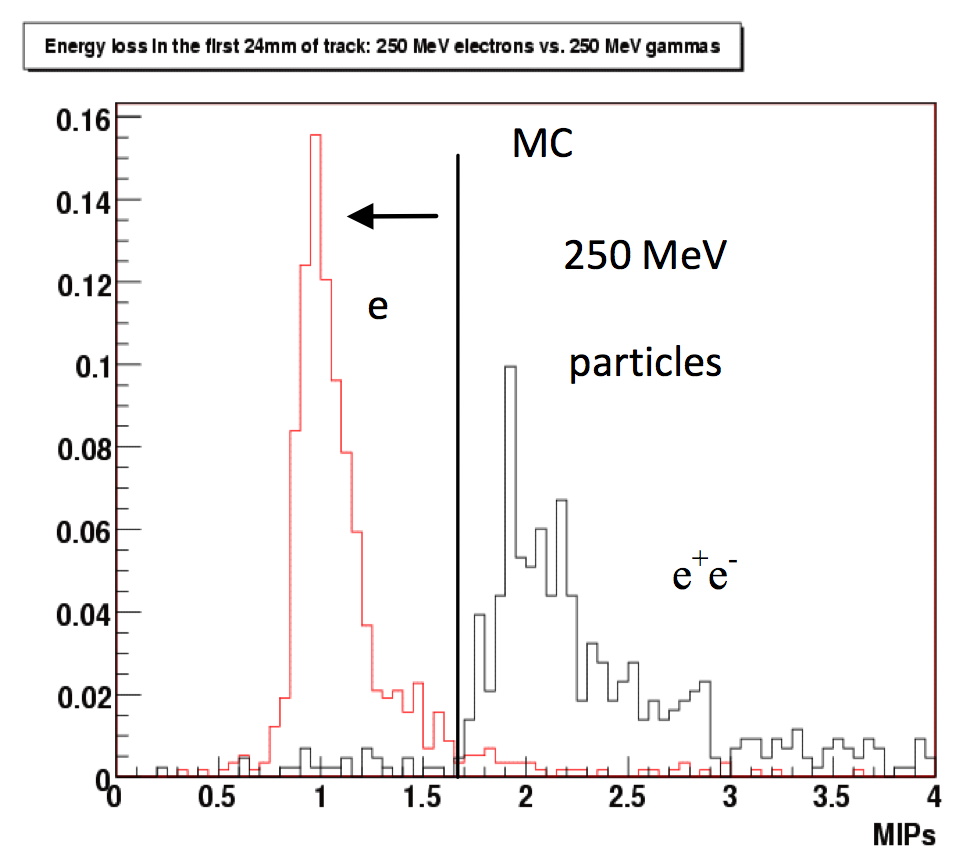
\includegraphics[width=0.9\textwidth]{Figures/UB_TDR_egamma_dedx.png} \\
\caption{\textit{Energy loss per unit length along the first 2.4 cm of simulated single electron showers (red) and single photon showers (black) in terms of minimally ionizing particle (MIP) energy in liquid argon (about 2.1 MeV/cm). Photons in general have twice the dE/dx of electrons at the start of their showers, stemming from pair production.}}\label{UB_TDR_egammadedx_fig}
\end{figure}

There are other important differences between the MiniBooNE detector and that of MicroBooNE which need to be considered when broaching the subject of estimating a sensitivity of a signal seen in MiniBooNE as it might be seen in MicroBooNE. These differences are summarized in Table \ref{UB_MB_comparison_table}. From the table it is clear that the event selection efficiency in MicroBooNE (not yet completely determined, but discussed in Section \ref{analysis_cut_descript_section}) will have to be much higher than that of MiniBooNE for two experiments to have comparable statistical significances. 

\begin{table}
\begin{tabular}{ |p{5cm}|p{3.5cm}|p{3.5cm}|  }
 \hline
 \multicolumn{3}{|c|}{MiniBooNE Compared to MicroBooNE} \\
 \hline
   & MiniBooNE & MicroBooNE \\
 \hline \hline
 Detector Technology & Cherenkov & LArTPC\\\hline
 Nominal POT & $6.46\times10^{20}$ & $6.6\times10^{20}$ \\\hline
 Active Volume Mass & 818 Tons & 89 Tons \\\hline
 Signal Selection Efficiency & 25\% & N/A \\\hline
 Readout Time Scale & nanoseconds & milliseconds \\\hline
 Distance from Neutrino Production Target & 541 m & 470 m \\\hline
 Target Material & $CH_2$ & Argon \\\hline
 e$\rightarrow\gamma$ Separation Power & None & High \\\hline
 Sensitive to Vertex Activity & No & Yes \\\hline
 \hline
\end{tabular}
\caption{\textit{A comparison of some of the important similarities and differences between the MiniBooNE detector and the MicroBooNE detector, which make the signal modeling in this sensitivity study difficult.}}\label{UB_MB_comparison_table}
\end{table}


\subsection{Past Sensitivity Studies}\label{georgia_scaling_description}

A preliminary attempt to scale the MiniBooNE backgrounds and excess to MicroBooNE is shown in Figure \ref{TDR_LEE_scaling_fig}, both under the assumption that the excess is due to an electron-like event (left) or due to a photon-like event (right) \cite{UBTDR}. Such a scaling is a subtle and difficult task because of the drastic differences between the MiniBooNE and MicroBooNE detectors, as described in the previous section.\\

\begin{figure}[ht!]
\centering
	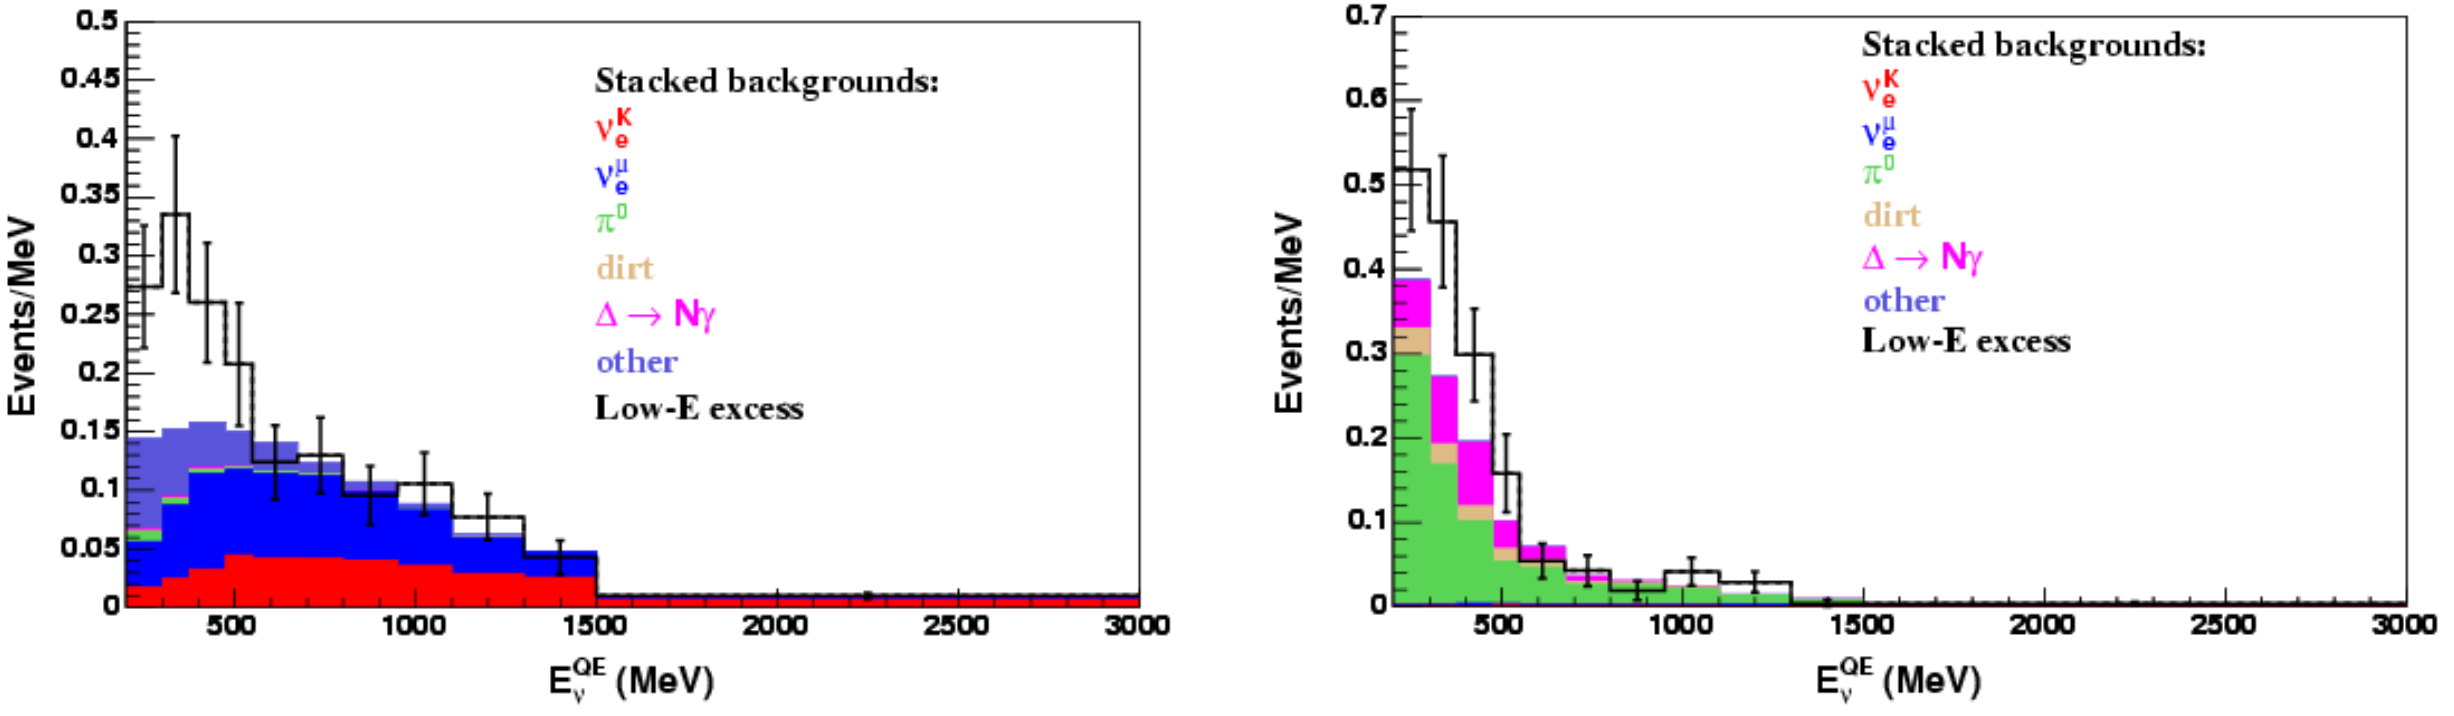
\includegraphics[width=0.9\textwidth]{Figures/TDR_LEE_scaling.png} \\
\caption{\textit{A preliminary attempt to scale the MiniBooNE backgrounds and excess to MicroBooNE both under the assumption that the excess is due to an electron-like event (left) or under a photon-like event (right). Stacked histograms show the expected background. Error bars indicate statistical uncertainty. The number of signal events, scaled from MiniBooNE for neutrino flux and fiducial volume, is the same in both plots (though dedicate electron-specific and photon-specific event selection cuts may show this to be unrealistic). Both plots assume $6.6 \times 10^20$ POT for the MicroBooNE 60 ton fiducial mass.}}\label{TDR_LEE_scaling_fig}
\end{figure}


This scaling assumes the electron/photon misidentification rate in MicroBooNE is 6\% (whereas it is 100\% for MiniBooNE). Also, event selection efficiencies in MicroBooNE are assumed to be exactly twice that of MiniBooNE because of the detector technology. This scaling procedure ignores other potentially important differences between MicroBooNE and MiniBooNE including differences in detector geometry (important for $\pi^0$ mis-identifications in which one photon escapes), flux differences (which are non-negligible despite the relative close physical proximity of the two detectors), event topology selection differences (MicroBooNE can see much more vertex activity than can MiniBooNE, especially when additional final state particles are below Cherenkov threshold), the differing cosmic rejection background efficiencies (MiniBooNE can reject cosmics more efficiently than MicroBooNE), cross section differences between argon and $CH_2$ arising from differing proton to neutron ratios, among other things. The analysis described later in this thesis will treat both of these assumptions with more rigor.\\

The resulting statistical significance from the aforementioned scaling after the nominal amount of data is taken in MicroBooNE ($6.6\times 10^{20}$ POT) is computed to be 5.7$\sigma$ under the single-electron excess hypothesis and 4.1$\sigma$ under the single-photon hypothesis. \\

The described scaling analysis is a very valuable tool, but making many assumptions is unavoidable to compute a sensitivity in this way. The next sections in this thesis describe a more rigorous analysis with the ultimate goal of computing MicroBooNE's sensitivity to the MiniBooNE low energy excess assuming specifically the single-electron hypothesis. In this analysis, actual signal and background events will be simulated in the MicroBooNE detector and event selection cuts and algorithms will be used to select them.














\section{Monte Carlo Simulation}

\subsection{Simulated Background Samples}\label{LEE_simulated_background_samples_section}
In this thesis analysis, both beam induced backgrounds and beam external backgrounds are simulated in the MicroBooNE cryostat. For beam-induced samples, the same flux predictions are used as were used in the MiniBooNE simulations (accounting for baseline and acceptance differences). The beam-induced samples come from full simulated BNB interactions with cross sections provided by GENIE \cite{GENIEsource}\footnote{Note that while MicroBooNE uses GENIE to simulate BNB interactions, MiniBooNE used NUANCE \cite{NUANCEsource}. Given the approach to determine the absolute normalization of the MiniBooNE excess as seen in MicroBooNE based on intrinsic $\nu_e$ rates (see Section \ref{MBLEESignalModeling_section}), differences between these two generators can be ignored.}. Beam-external samples (cosmics) come from simulated CORSIKA generated \cite{CORSIKAsource} cosmic rays that pass through the cryostat. Cosmic rays passing through other portions of the detector hall but not the cryostat result in negligible backgrounds in this $\nu_e$ search. The passage of all particles through the detector volume is simulated by the {\sc GEANT4} package \cite{GEANT4source}. 

\subsection{Reconstruction}
In general, the output of an automated reconstruction chain in a LArTPC consists of reconstructed optical hits which come from the PMT signals, and reconstructed wire hits which come from drift electron ionization signals on the induction and collection plane wires. Reconstruction algorithms cluster the latter hits on each wire plane into those corresponding to individual particles, then match clusters from different wire planes to form 3D reconstructed objects. The wire planes provide two of the three dimensions, and matching clusters to optical hits on the PMTs provide the third (drift) dimension. These reconstructed objects are either thin, straight tracks (which come from particles like muons, charged pions, and protons) or more fuzzy cone-shaped showers, which come from higher energy electrons or photons. Ideally this analysis would be done using these reconstructed objects. In this way, the same event selection  methods could be used on data as are used in simulation. While automatic track reconstruction can currently be performed at an adequate level, the difficulties involved in shower reconstruction (which is particularly important to tag and study $\nu_e^{CC}$ events) have yet to be overcome.\\

For these reasons, this simulation-only study is done with objects that are not automatically reconstructed from wire and PMT signals, but instead from truth-based energy depositions in the detector. In general, these objects represent what would be reconstructed from wire and PMT signals if the reconstruction algorithms performed perfectly. Therefore, this is referred to as ``perfect reconstruction'' and the details of it are discussed in the next section. 

\subsubsection{``Perfect Reconstruction''}\label{perfectreco_section}
% Description of what {\sc MCTracks} and {\sc MCShowers} are, how they're made, etc. Make it clear that they are the input to the event reconstruction algorithms. Also make it clear that this entire sensitivity study is done only with these objects; no real automated reconstruction is covered (which is why no results on data are shown).
While a simulation-only study using real automated reconstruction would be ideal, such a study using ``perfect reconstruction'' is incredibly valuable; it is a step forward from the aforementioned simple scaling study (Section \ref{georgia_scaling_description}), and the event selection cuts and algorithms designed in this study can be used out-of-the-box on automated reconstructed objects once they become available. Additionally, the ``perfect reconstruction'' can be tuned to more realistically represent what automated reconstruction might be capable of, for example by smearing the energy of objects or emulating realistic reconstruction efficiencies. This will provide the important estimate of uncertainties arising from the imperfect automated reconstruction.\\

As mentioned earlier, the final 3D reconstructed objects formed from wire plane signals and PMT signals are referred to as tracks or showers. Tracks are close to straight lines in three dimensions, while showers are fuzzier and generally cone-shaped in three dimensions. The ``perfect reconstruction'' analogs to tracks and showers are referred to as {\sc MCTracks} and {\sc MCShowers}. They are created from simulated {\sc GEANT4} 3D energy depositions in the detector volume. {\sc GEANT4} outputs 3D energy depositions in the detector, along with truth information about which parent particles deposited this energy. {\sc MCShowers} and {\sc MCTracks} are 3D objects which are formed by grouping energy depositions based on parent particles. Whether a particle in {\sc GEANT4} becomes an {\sc MCShower} or an {\sc MCTrack} is based on truth PDG (for example, electrons always form {\sc MCShower}s\footnote{Despite the fact that electrons behave more like tracks below the critical energy, which is on the order of 40 MeV in liquid argon} and muons always form {\sc MCTrack}s). Only the energy deposited by particles \textit{within the TPC} is used to form these ``perfect reconstructed'' objects, which is in line with them representing actual reconstructible quantities (no ionization outside of the TPC is reconstructible).\\

% To clarify, consider the following simulated interaction: a $\nu_e$ charged current interaction in which the final state particles are an electron, a charged pion, a neutral pion, and two protons. The charged pion travels until it stops, where it decays into a muon, which then travels and decays into an electron. The generated ``perfect reconstruction'' objects in the event will be four {\sc MCShower}s (for the electron exiting the interaction, the electron from the muon decay, and one for each photon originating from the neutral pion decay) and four {\sc MCTracks} (one for the charged pion, one for the muon, and one for each proton).\\

{\sc MCTracks} consist of a series of ordered 3D trajectory points, each corresponding to an energy deposition in the detector. {\sc MCShowers} have the following attributes: 3D start point where the first energy from the parent particle is deposited, 3D direction which is computed by fitting a line in 3D to all of the deposited energy from the parent particle, and dE/dx computed from the energy depositions along the first few centimeters of the shower. These ``perfectly reconstructed'' tracks and showers ({\sc MCTracks} and {\sc MCShowers}) serve as the input to the event selection algorithms, just as automated reconstructed tracks and showers (with the same attributes) would in real data.\\




\section{Event Selection}\label{LEE_eventselection_section}
This section describes the algorithms and cuts used to identify $\nu_e^{CC}$ interactions, given as input the ``perfect reconstructed'' {\sc MCTracks} and {\sc MCShowers} from simulated triggered events in MicroBooNE\footnote{Note that these cuts and algorithms could use automatically reconstructed tracks and showers, and therefore could be run both on simulation and data, if the quality of track and shower reconstruction was high enough.}. Note that while the event selection algorithms are designed to identify $\nu_e^{CC}$ inclusive interactions (which may involve pions in the final state, for example), ultimately only the $\nu_e^{CCQE}$ events (with only one electron and protons in the final state) are used in the final sensitivity estimates.\\

To select $\nu_e^{CC}$ interactions in MicroBooNE, a series of nine algorithms are run, each with a specific goal in mind; they either identify background topologies in order to remove them, or they identify the signal $\nu_e^{CC}$ topology. For example, one algorithm identifies {\sc MCShowers} which are likely delta rays originating from tracks. Once identified, these {\sc MCShowers} are no longer candidate $\nu_e^{CCQE}$ electrons. Another algorithm identifies pairs of showers that are likely from $\pi^0$ decays (by using the dE/dx of those showers, and requiring they back-project to a common origin) in order to remove them from the pool of candidate $\nu_e^{CC}$ electrons. Another algorithm tags through-going tracks as cosmic in origin, ensuring they will not be associated with a neutrino interaction.\\

The two most important event selection algorithms for this analysis are named ``AlgoEMPart'' (which handles the electron/photon discrimination) and ``AlgoSingleE'' (which is the algorithm responsible for locating the $\nu_e^{CC}$ topology and associating all tracks and showers together for eventual energy reconstruction and analysis). These two algorithms are discussed in detail in the following two subsections. The remaining seven event reconstruction algorithms are discussed in detail in the appendices of this thesis (XXX will add this later). Note that at the end of the chain of event selection algorithms, a sample of candidate $\nu_e^{CC}$ events is tagged. These events are the subject to further cuts both to mitigate some backgrounds that the event selection algorithms missed, and more importantly to pick specifically $\nu_e^{CCQE}$ events so as to make the eventual comparison to the MiniBooNE excess, since MiniBooNE searched for $\nu_e^{CCQE}$ events, not $\nu_e^{CC}$.

% This section describes how we take reconstructed objects (tracks and showers) and identify nue interactions. Mention that the analysis framework has many algorithms that each serve a specific purpose. Briefly mention the algorithms by name and what they're intended to do. Include the flowchart figure from the APS technote listing all the algorithms and the order in which they are executed. The following sections will describe in more detail the important ones. 

\subsection{Electron/Photon Separation Algorithm}\label{algoempart_section}
% This is the algorithm (AlgoEMPart) that uses the reconstructed dE/dx and conversion distance to form a likelihood that a shower is electron like or photon like. It's one of the most important and should be described in detail. Include some figures showing performance of this algorithm.
Electron/photon separation based on dE/dx at the start of showers is done through an algorithm called ``AlgoEMPart". This algorithm uses trained likelihood distributions which input dE/dx and return the likelihood that the shower is electron-like, or photon-like. If a conversion distance (the distance between the reconstructed start point of the shower and the first energy deposition of the shower) is known, it will incorporate that into its likelihood as well. This additional handle is powerful because in general an electron shower will have a near-zero conversion distance, while a photon shower will often have a conversion distance of several centimeters. The algorithm's likelihood is configured with parameters output by a RooFit \cite{ROOFITsource} minimization routine. The RooFit routine is trained on simulated single electron and single photon {\sc MCShowers}. In general, this algorithm computes both the likelihood that an {\sc MCShower} is an electron and that it is a photon, and determines the identity of the particle to be the one with the larger likelihood.\\

There are two likelihood functions that may be used. If a shower can independently be associated with a neutrino interaction vertex, the algorithm will use a 2D likelihood function that includes both dE/dx and radiation length information. If an algorithm cannot associate a vertex with a shower, there is a 1D likelihood function that can be used with only dE/dx information. The 1D likelihood function is composed of a Gaussian plus a landau distribution for dE/dx, and the 2D likelihood function also includes an exponential function for radiation length. Any potential energy dependence on dE/dx or conversion distance is not included in these likelihoods. The twelve trained input parameters include mean and sigma values for the Gaussian distributions, the MPV and sigma values for the landau distributions, the fractional area difference between the Gaussian and landau distributions, and the radiation length parameter (six parameters for electrons, six parameters for photons). When training, input parameters for each sample (electron, photon) are the {\sc MCShower} computed dE/dx as well as the truth-level creation vertex of the particle. The training results on ``perfect reconstruction'' electron and photon showers are shown in Figure \ref{empart_perfectreco_performance_fig2}.%, then zoomed in in Figure \ref{empart_perfectreco_performance_fig3}.

\begin{figure}[ht!]
\centering
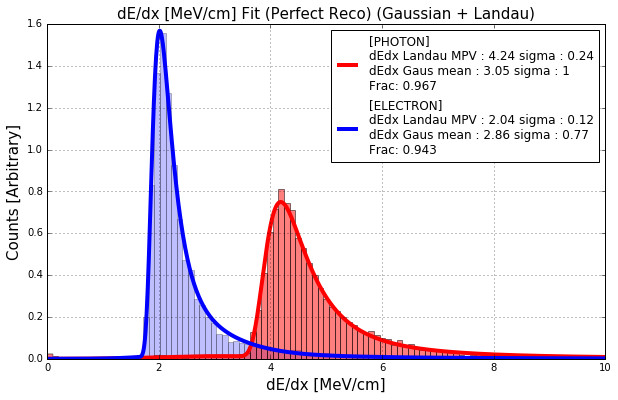
\includegraphics[width=0.9\textwidth]{Figures/EMPartTraining/mc_trained/dEdx_Selected_both.png}\\
\caption{\textit{AlgoEMPart training results on perfect reconstructed electron showers and on perfect reconstructed photon showers as described in Section \ref{empart_perfectreco_performance}: 1D landau + Gaussian fit to dE/dx.}}
\label{empart_perfectreco_performance_fig2}
\end{figure}

% \begin{figure}[ht!]
% \centering
% 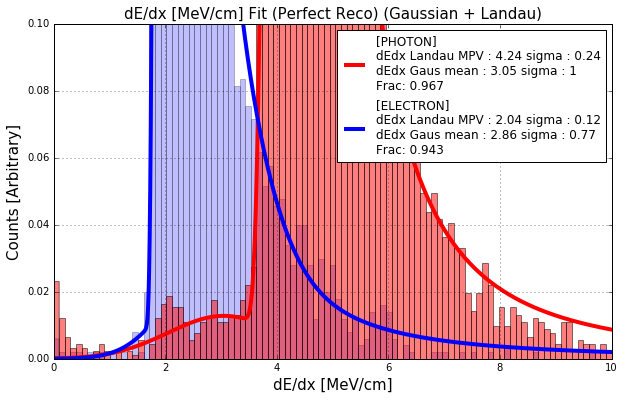
\includegraphics[width=0.9\textwidth]{Figures/EMPartTraining/mc_trained/dEdx_Selected_both_zoomed.png}\\
% \caption{\textit{The same plot as shown in Figure \ref{empart_perfectreco_performance_fig2}, but zoomed in along the y-axis to show the Compton peak in the photon sample, as well as the pileup of very low dE/dx values for photons (due to soft Compton scatters as described in Section \ref{perfectreco_section}).}}
% \label{empart_perfectreco_performance_fig3}
% \end{figure}

\subsubsection{Performance}\label{empart_perfectreco_performance}
The performance of this algorithm on ``perfect reconstruction" is computed by using samples of single electron showers and single photon showers generated isotropically between 0.05 and 2 GeV, and selecting those events where greater than 90\% of the shower's energy is contained within the TPC. The algorithm's likelihood is trained using this sample (integrated over the full energy range of the showers). The efficiency to tag electrons and photons both with the 1D and the 2D likelihood are enumerated below.
\begin{enumerate}
\item Using \textit{only dE/dx} information, the efficiency (over all energies) to select a single electron is 93\%, while the MID efficiency to tag the electron as a photon is 7\%. 
\item Using \textit{only dE/dx} information, the efficiency to select a single photon is 97.3\%, while the MID efficiency to tag the photon as an electron is 2.7\%.
\item Using \textit{both dE/dx and radiation length} information (using the true creation point of photons), the efficiency to select a single electron is 99.7\%, while the MID efficiency to tag the electron as a photon is 0.3\%. 
\item Using \textit{both dE/dx and radiation length} information (using the true creation point of photons), the efficiency to select a single photon is 98.1\%, while the MID efficiency to tag the photon as an electron is 1.9\%.
\end{enumerate}


The 1D likelihood to determine if a shower is electron-like or photon-like is shown in Figure \ref{empart_perfectreco_performance_fig4}. The likelihood that a shower with a given dE/dx is electron-like is computed by the ratio of the 1D electron-like probability distribution function (PDF) value for that dE/dx (shown non-normalized in Figure \ref{empart_perfectreco_performance_fig2}) to the sum of the electron-like PDF value for that dE/dx and the photon-like PDF value for that dE/dx (shown non-normalized in Figure \ref{empart_perfectreco_performance_fig2} as well) (Equation \ref{1D_dedx_likelihood_eqtn}). 

\begin{equation}\label{1D_dedx_likelihood_eqtn}
LL_e=\frac{e_{dE/dx}^{PDF}(\frac{dE}{dx})}{ e_{dE/dx}^{PDF}(\frac{dE}{dx}) + g_{dE/dx}^{PDF}(\frac{dE}{dx}) }
\end{equation}
where $e_{dE/dx}^{PDF}(\frac{dE}{dx})$ represents the electron dE/dx PDF function (shown non-normalized in Figure \ref{empart_perfectreco_performance_fig2}) evaluated at a dE/dx value $\frac{dE}{dx}$ and $g_{dE/dx}^{PDF}(\frac{dE}{dx})$ represents the photon dE/dx PDF function (also shown non-normalized in Figure \ref{empart_perfectreco_performance_fig2}) evaluated at a dE/dx value $\frac{dE}{dx}$. The likelihood that a shower with a given dE/dx is photon-like is similarly computed but with the photon-like PDF value for that dE/dx in the numerator.\\

The 2D likelihood including both dE/dx and conversion distance is shown in Figure \ref{empart_perfectreco_performance_fig1}. The likelihood that a shower with a given dE/dx value, $\frac{dE}{dx}$ and a given conversion distance value, $d$ is electron-like is computed as follows: 
\begin{equation}\label{2D_likelihood_eqtn}
LL_e=log( \frac{e_{dE/dx}^{PDF}(\frac{dE}{dx}) * e_{conv}^{PDF}(d)}{g_{dE/dx}^{PDF}(\frac{dE}{dx}) * g_{conv}^{PDF}(d)} )
\end{equation}
where $e_{dE/dx}^{PDF}(\frac{dE}{dx})$ represents the electron dE/dx PDF function (shown non-normalized in Figure \ref{empart_perfectreco_performance_fig2}) evaluated at a dE/dx value, $\frac{dE}{dx}$, $e_{conv}^{PDF}(d)$ represents the electron conversion distance PDF function (shown non-normalized in Figure \ref{empart_perfectreco_performance_fig6}) evaluated at a conversion distance value, $d$, $g_{dE/dx}^{PDF}(\frac{dE}{dx})$ represents the photon dE/dx PDF function (shown non-normalized in Figure \ref{empart_perfectreco_performance_fig3}) evaluated at a dE/dx value, $\frac{dE}{dx}$, $g_{conv}^{PDF}(d)$ represents the photon conversion distance PDF function (shown non-normalized in Figure \ref{empart_perfectreco_performance_fig7}) evaluated at a conversion distance value, $d$. The likelihood that the same shower is photon-like is simply the inverse of Equation \ref{2D_likelihood_eqtn}.\\



\begin{figure}[ht!]
\centering
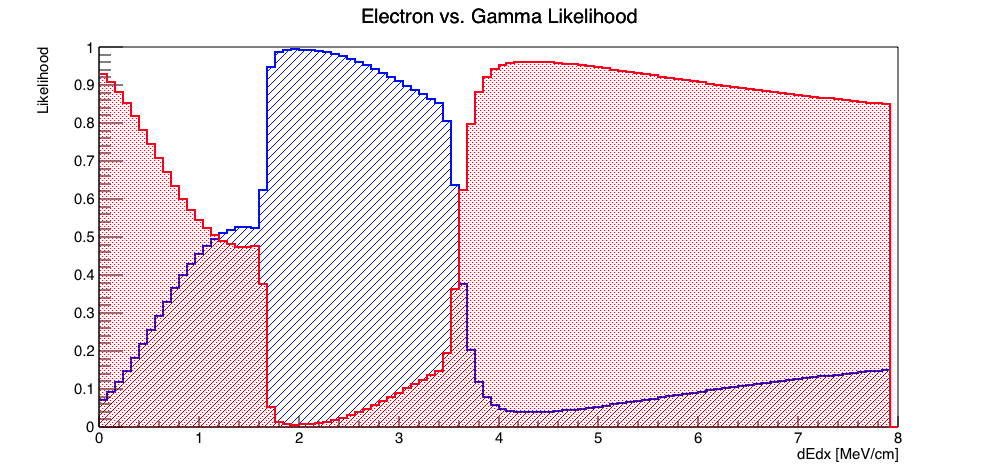
\includegraphics[width=0.9\textwidth]{Figures/EMPartTraining/mc_trained/Likelihood_dEdx.png}\\
\caption{\textit{AlgoEMPart: Computed 1D likelihood vs dE/dx: red is photon, blue is electron. How the likelihood is computed is described in Section \ref{empart_perfectreco_performance}.}}
\label{empart_perfectreco_performance_fig4}
\end{figure}


\begin{figure}[ht!]
\centering
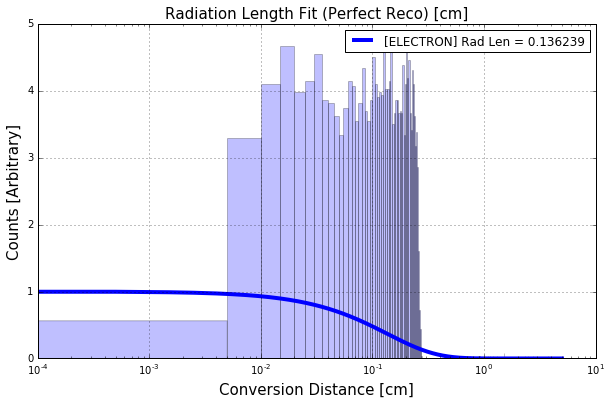
\includegraphics[width=0.9\textwidth]{Figures/EMPartTraining/mc_trained/RadLength_Selected_e.png}\\
\caption{\textit{AlgoEMPart training results on perfect reconstructed electron showers as described in Section \ref{empart_perfectreco_performance}: Radiation length fit to single electron showers. Note the poor quality of the fit as the electron conversion distance for ``perfect reconstruction'' does not follow an exponential distribution; all conversion distances are below 0.3 centimeters.}}
\label{empart_perfectreco_performance_fig6}
\end{figure}

\begin{figure}[ht!]
\centering
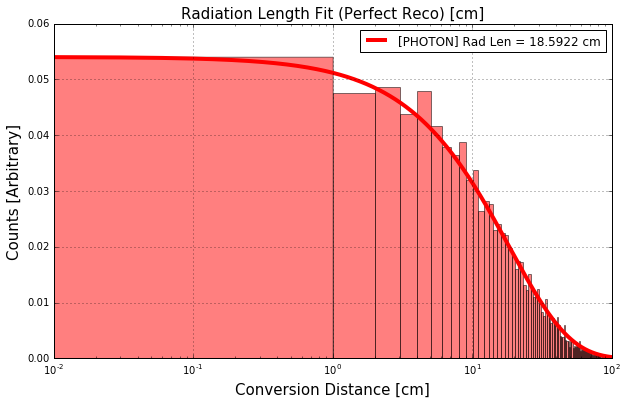
\includegraphics[width=0.9\textwidth]{Figures/EMPartTraining/mc_trained/RadLength_Selected_g.png}\\
\caption{\textit{AlgoEMPart training results on perfect reconstructed photon showers as described in Section \ref{empart_perfectreco_performance}: Radiation length fit to single photon showers.}}
\label{empart_perfectreco_performance_fig7}
\end{figure}


\begin{figure}[ht!]
\centering
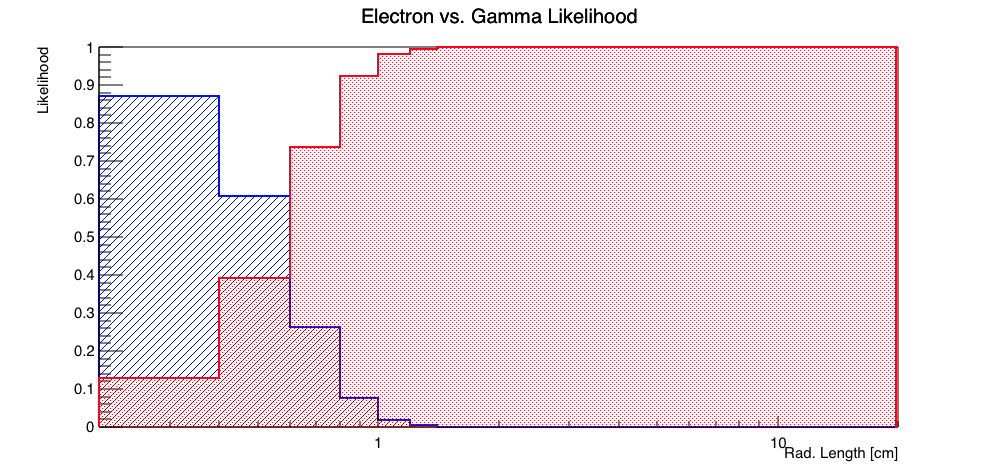
\includegraphics[width=0.9\textwidth]{Figures/EMPartTraining/mc_trained/Likelihood_radLen.png}\\
\caption{\textit{AlgoEMPart: Computed 1D likelihood vs conversion distance (integrated over all energies): red is photon, blue is electron. How the likelihood is computed is described in Section \ref{empart_perfectreco_performance}.}}
\label{empart_perfectreco_performance_fig5}
\end{figure}

\begin{figure}[ht!]
\centering
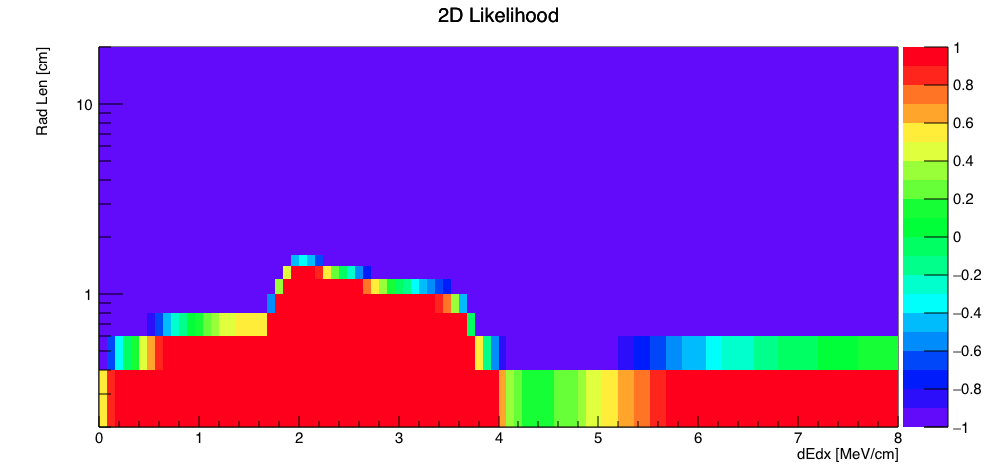
\includegraphics[width=0.9\textwidth]{Figures/EMPartTraining/mc_trained/2DRatio.png}\\
\caption{\textit{AlgoEMPart training results on perfect reconstructed electron and photon showers as described in Section \ref{empart_perfectreco_performance} integrated over all energies: 2D likelihood distribution (radiation length vs. dE/dx). Low values of likelihood (purple) correspond to photon-like, high values (red) correspond to electron-like.}}
\label{empart_perfectreco_performance_fig1}
\end{figure}























































\subsection{Signal Selection Algorithm}

The purpose of this algorithm is to reconstruct events with $\nu_e^{CC}$ inclusive type topologies. These topologies involve a single electron at a neutrino interaction vertex, with any number of protons, charged or neutral pions, or anything else additionally exiting the vertex. Later on, the sample of selected events will be subjected to further cuts to select only $\nu_e^{CCQE}$ topologies by rejecting events with pions in the final state. This algorithm uses likelihoods provided by the previously described ``AlgoEMPart'' (Section \ref{algoempart_section}) to determine if a shower is an electron or a photon. This algorithm begins by looping over all candidate $\nu_e^{CC}$ electron showers in the event that have not been removed by upstream cosmic and $\pi^0$ tagging algorithms. Figure \ref{algosinglee_flowchart_fig} is a flowchart depicting decision tree this algorithm uses for each candidate $\nu_e^{CC}$ electron shower. If the algorithm reaches the bottom of the flowchart, that shower is determined to be from a $\nu_e^{CC}$ interaction and the event is saved to be included in analysis. The flowchart refers to determining if two showers are correlated and determining if a shower is correlated with the start of a track. A schematic which diagrams how these determinations are made is shown in Figure \ref{algosinglee_cartoon_fig}. A list of configurable parameters and their chosen cut values can be found in Table \ref{algosinglee_table}. A more detailed description of Figure \ref{algosinglee_flowchart_fig} is given in the following paragraphs.\\


\begin{figure}[ht!]
\centering
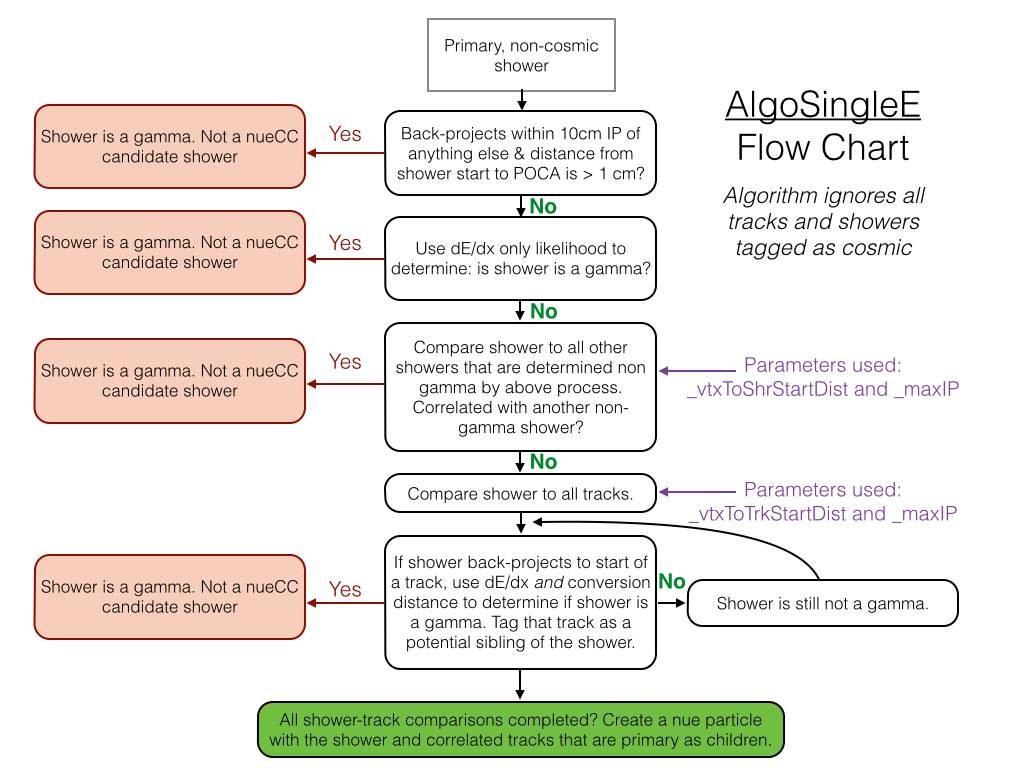
\includegraphics[width=150mm]{Figures/algosinglee_flowchart.png}\\
\caption{\textit{A flowchart depicting decisions the algorithm makes for each primary, non-cosmic shower. If the algorithm gets to the bottom of the flowchart, that shower was determined to be from a $\nu_e^{CC}$ interaction, and a $\nu_e$ particle is created.}}
\label{algosinglee_flowchart_fig}
\end{figure}

\begin{figure}[ht!]
\centering
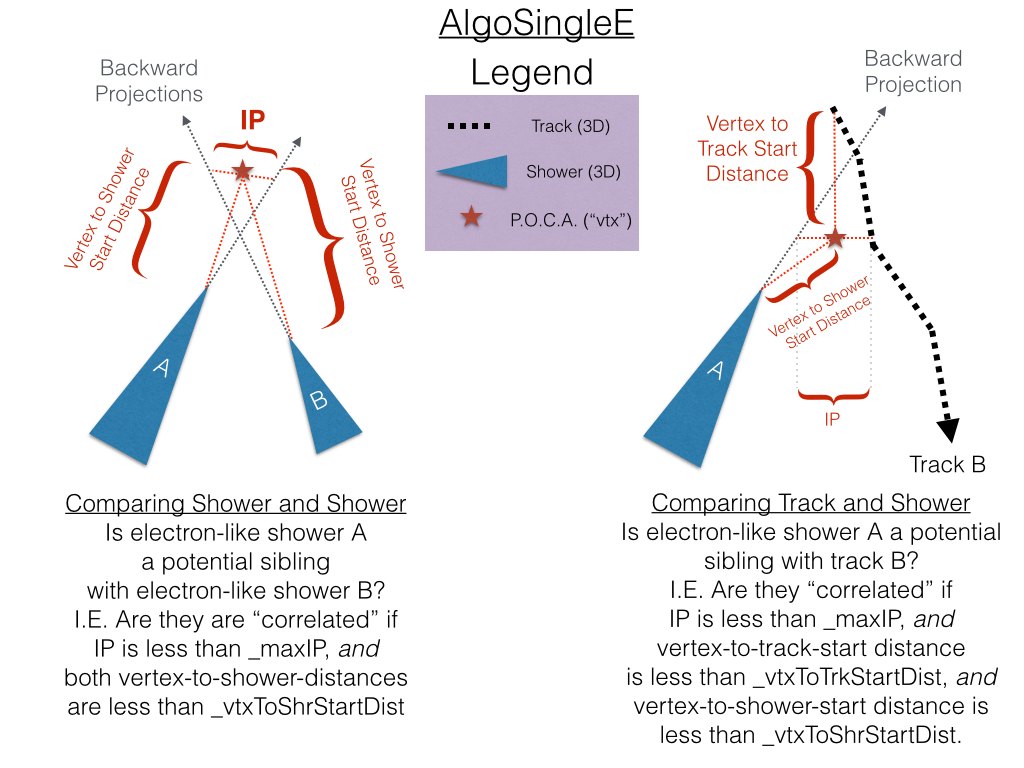
\includegraphics[width=150mm]{Figures/algosinglee_cartoon.png}\\
\caption{\textit{Schematic cartoons indicating how the signal selection algorithm makes decisions determining if two reconstructed showers are correlated, and if a reconstructed shower is correlated with a reconstructed track (as described in Figure \ref{algosinglee_flowchart_fig}).}}
\label{algosinglee_cartoon_fig}
\end{figure}

For each primary, non-cosmic shower (``shower A''in Figure \ref{algosinglee_cartoon_fig}), this algorithm computes the point of closest approach and impact parameter between the shower's back-projection and to all other tracks, as well as to all other shower back-projections. If the smallest impact parameter (IP) is less than 10 centimeters and the distance between the shower's start point and the point of closest approach is greater than 1 centimeter, the algorithm assumes this shower is a photon and it rejects the shower as a potential $\nu_e^{CC}$ shower, without any dE/dx considerations\footnote{Note that for $\nu_e^{CC}$ interactions and ``perfect reconstruction'', these impact parameters and points of closest approach between the $\nu_e^{CC}$ electron shower and other tracks in the event are incredibly small (sub centimeter). The cut values are chosen to be much larger to simulate estimated automatic track and shower reconstruction resolutions.}. Otherwise, the algorithm continues by using AlgoEMPart's trained likelihood function to determine based on dE/dx alone whether this shower is gamma-like and should therefore be ignored.\\

Assuming this potential $\nu_e^{CC}$ shower has so far been found to be electron-like, the algorithm then compares the shower to all other showers in the event that are not marked as cosmic, and are not already reconstructed to be the descendant of another particle. The purpose of this portion of the code is to enforce that the topology of interest includes a \textit{single electron} exiting the neutrino interaction. If any other electron-like showers are nearby that could be potentially correlated, the shower is rejected as a candidate $\nu_e^{CC}$ electron.\\

The candidate shower is then compared to every track in the event that has not been tagged as cosmic to look for correlations between the potential $\nu_e^{CC}$ electron and tracks (Figure \ref{algosinglee_cartoon_fig}). The topology of interest allows for the electron to point back to the \textit{start} of a track, but \textit{not} to the middle or end of a track (as these showers are likely delta rays or Michel electrons). At this point, the code again uses a likelihood from AlgoEMPart to determine if the shower is still electron-like, this time using both the shower's dE/dx \textit{and} the distance between the shower start and the computed P.O.C.A. as a radiation length. This is a more powerful discrimination to determine if the shower remains electron-like. If the shower remains electron-like and is found to be correlated with the start of a track, the track is stored as associated with another final state particle of the $\nu_e^{CC}$ interaction. The energy of this track will later be included in the reconstructed neutrino energy.\\

At this point, a $\nu_e^{CC}$ event has been found, and the shower and any associated tracks are stored to be included in the sensitivity analysis.

\subsubsection{Configurable Parameters}
The configurable parameters for this algorithm are summarized in the Table \ref{algosinglee_table}. Note that with ``perfect reconstructed'' showers, these distances are always very small (less than 0.1 centimeters), so these values were chosen to introduce some realism into the algorithm by estimating detector resolutions.\\\\

\begin{table}
\begin{tabular}{ |p{8cm}|p{1.5cm}|  }
 \hline
 \multicolumn{2}{|c|}{AlgoSingleE: Parameters} \\
 \hline
 Parameter Name &  Cut Value \\
 \hline \hline
 Use Radiation Length &  True\\\hline
 
 Max Vertex-to-Track-Start Distance & 1 cm \\\hline

 Min Vertex-to-Shower-Start Distance & 50 cm \\\hline

 Maximum IP & 1 cm \\\hline

 \hline
\end{tabular}
\caption{\textit{The list of configurable parameters and their values used in the AlgoSingleE $\nu_e^{CC}$ signal selection algorithm. Note that for $\nu_e^{CC}$ interactions and ``perfect reconstruction'', these actual values the distance-based parameters represent are incredibly small (sub centimeter). The cut values are chosen to be much larger to simulate estimated automatic track and shower reconstruction resolutions.}}\label{algosinglee_table}
\end{table}










\subsection{Energy Reconstruction}\label{LEE_EnergyReco_section}
%Description of the energy definition. Mention that it is different than the CCQE energy definition MiniBooNE used. Include a figure of Ereco vs Etrue for the intrisic nue sample.

With the candidate $\nu_e^{CC}$ interactions identified, the neutrino energy is reconstructed in two ways. First, the angle and energy of the selected $\nu_e^{CC}$ electron is used to compute an energy, $E_\nu^{CCQE}$ from the CCQE formula, Equation \ref{MB_CCQE_formula}. This is the same energy definition that is used in the MiniBooNE oscillation analysis. Note that this energy is only valid for truly $\nu_e^{CCQE}$ interactions, which are a subset of the selected $\nu_e^{CC}$ sample.\\

An additional, more accurate energy estimation, $E_{\text{calo}}$ is calculated by looping over all particles tagged as descendants of the reconstructed $\nu_e$ and adding up their deposited energies. For $\nu_e^{CC}$ events, this amounts to adding the deposited energy of the electron shower, along with the deposited energies from all protons exiting the interaction vertex, and energies from charged and neutral pions exiting the vertex (adding the pion masses). Additionally the electron mass is added, though this changes the calculated energy negligibly. Plots describing the neutrino reconstruction performance for correctly identified $\nu_e^{CCQE}$ interactions can be seen in Figures \ref{energy_smear_plot_fig} and \ref{energy_res_plot_fig}. The energy resolution for true neutrino energies below 500 MeV is on the order of 15\%, and the bias indicates that the energy reconstruction method tends to underestimate true neutrino energy by about 25\%. Note that this bias is computed as the mean reconstructed energy of all events in a specific true energy bin rather than the center of a Gaussian fit to the central distribution of events, so the bias is skewed down by outliers.

\begin{figure}[ht!]
\centering
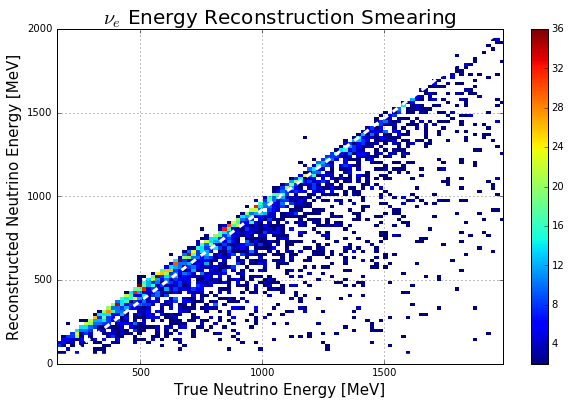
\includegraphics[width=0.9\textwidth]{Figures/LEE_EnergySmear_WithAnalysisCuts.png}\\%Figures/background_technical/nue/energy_smear_plot.png}
\caption{\textit{Reconstructed neutrino energy as described in Section \ref{LEE_EnergyReco_section} versus true neutrino energy. This plot was made from ``perfect reconstruction'' objects in correctly identified $\nu_e^{CCQE}$ events after all final analysis cuts were placed.}}
\label{energy_smear_plot_fig}
\end{figure}

\begin{figure}[ht!]
\centering
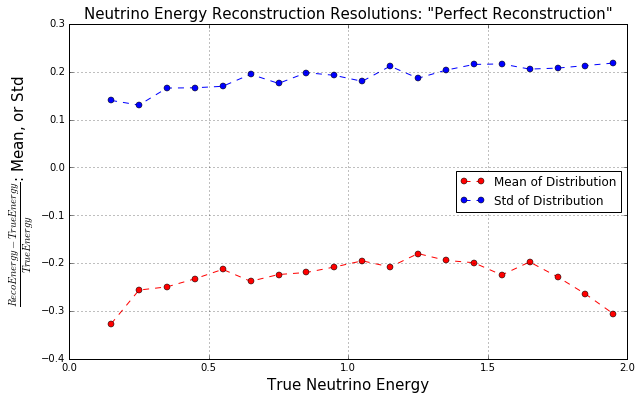
\includegraphics[width=0.9\textwidth]{Figures/LEE_EnergyRes_WithAnalysisCuts.png}\\%Figures/background_technical/nue/energy_res_plot.png}
\caption{\textit{A neutrino energy resolution and bias plot. This is created by binning Figure \ref{energy_smear_plot_fig} in true neutrino energy and making a distribution of (Reco Energy - True Energy)/(True Energy). For each bin, the mean (red) and standard deviation (blue) are plotted in the above figure. This plot was made from ``perfect reconstruction'' objects in correctly identified $\nu_e^{CCQE}$ events after all final analysis cuts were placed.}}
\label{energy_res_plot_fig}
\end{figure}

\section{Backgrounds}

\subsection{Background Topologies}\label{LEEbackgroundtopologiessection}

\subsubsection{Intrinsic $\nu_e$}
The intrinsic $\nu_e^{CCQE}$ background comes from $\nu_e^{CCQE}$ interactions from Booster Neutrino Beam (BNB) electron neutrinos. The topology of these events involve one electron in the final state, with any number of protons exiting the interaction vertex, but no pions or muons exiting the interaction vertex. Neutral particles included in hadronic activity are also ignored as they are invisible from the point of view of a LArTPC. This background is irreducible for a $\nu_e^{CCQE}$ appearance search, and the dominant background in this analysis. These intrinsic $\nu_e$s in the relevant low energy region are mostly from muon decay in the beam line. The flux uncertainty can be constrained by a parallel $\nu_\mu$ analysis, as was done in MiniBooNE. While constraining $\nu_e$ from muon decay in the beam line with a parallel $\nu_\mu$ analysis, constraining $\nu_e$ from kaon decay in the beam line is discussed in the next chapter of this thesis.

\subsubsection{Intrinsic $\nu_\mu$}
The intrinsic $\nu_\mu$ background comes from $\nu_\mu$CC interactions from BNB muon neutrinos. Despite the enormous ratio of $\nu_\mu$CC events to $\nu_e^{CC}$ events, this is a sub-dominant background in this analysis. Potential sources of mis-identifications (MIDs) must always involve at least one shower, and there should not be a track recognized as a muon exiting the interaction vertex. For this reason, most $\nu_\mu$CC MIDs are from either
\begin{enumerate}
\item $\mu$ decay electrons (either in flight, or at rest when the energy of the electron is in the very high end of the Michel spectrum), or 
\item $\nu_\mu$CC events with a neutral pion in the final state. 
\end{enumerate}
The first MID source is suppressed because the electron points back to the end of the muon track and therefore is generally tagged by event selection algorithms. Additionally, these events are removed if the outgoing track is correctly identified as a muon. However, this background may be more prominent if the muon reconstructed track direction gets flipped (after which, correct identification of the muon track becomes more difficult, and the electron would point back to the \textit{start} of the track). The effect of flipping this track is not included in this analysis, but the impact is expected to be small because there are several handles on track directionality in LArTPCs including from multiple Coulomb scattering and delta rays.\\

The second MID source occurs when one of the photons of the neutral pion decay from a $\nu_\mu^{CC}\pi^0$ interaction is misidentified as an electron. This background is greatly suppressed because the dE/dx of the shower should be photon-like, and the shower points back towards the muon start point. The fact that the shower is displaced from the muon start point allows for a photon-like likelihood calculation using both the shower dE/dx and the radiation length, which is a more powerful discrimination tool to tag the shower as being from a photon (as described in Section \ref{algoempart_section}). Additionally, if the second photon converts inside of the detector, this provides another handle that the shower is from a neutral pion.

\subsubsection{Intrinsic Neutral Current (NC)}
The intrinsic NC background comes from neutral current interactions by any neutrino type from the beam. In these interactions, the neutrino interacts with the exchange of a neutral $Z$ boson, and the neutrino carries off some energy and momentum as it exits the detector. This fact (that the summed momenta of all children from the interaction won't point along the beam direction) can be leveraged to mitigate these backgrounds. The predominant NC background for the low energy excess analysis are $\nu_x$ (mostly $\nu_\mu$) interactions with a neutral pion in the final state. This was by far the most dominant background in the MiniBooNE $\nu_e$ appearance analysis (see Figure \ref{MB_published_stackedhisto_fig}). In this topology, one of the photons from the neutral pion decay is mis-identified as an electron coming from a $\nu_e^{CC}$ interaction. This background is significantly mitigated when both photons convert inside of the detector. In that case, the presence of two showers pointing back to a common origin allows for the event to be rejected.\\

An additional NC background topology is NC $\Delta \rightarrow N\gamma$, though this background is sub-dominant to the aforementioned neutral pion decays.

\subsubsection{Beam-Induced, TPC External (``B.I.T.E.'')}\label{BITE_physics_section}
This background comes from beam neutrino interactions that occur outside of the TPC volume, but inside of the cryostat volume (including the cryostat walls). By volume (and mass), this region is roughly half of the volume of the entire cryostat. The predominant topology for this background are neutrino interactions involving a neutral pion in the final state where only one photon from the pion decay converts inside of the TPC. Since this photon may not point back to any other reconstructed objects in the TPC, only its dE/dx can be used in the electron/photon separation likelihood which provides less discrimination power than if a radiation length could be used as well. Note that this analysis does not explicitly ask for a visible hadronic vertex, otherwise many of these backgrounds would be mitigated (though much of the signal would be mitigated as well). In this analysis, this background can be mitigated with cuts like backward-projected distance to a TPC wall, since they are all coming from outside of the TPC.

\subsubsection{Cosmic}
This background comes from cosmic rays that pass through the detector. The relatively high cosmic rate inside of the detector hall makes for on the order of tens of cosmic rays passing through the detector during the full readout window. Since the readout window is several milliseconds (since this is the time scale with which ionizations drift across the width of the TPC) and the cosmic rate through the detector is on the order of kHz, several cosmics arrive during each readout window. Measured reconstructed cosmics for a full readout window of 4.8 $ms$ are shown in Figure \ref{UB_publicplot_3dcosmics}.\\


\begin{figure}[ht!]
\centering
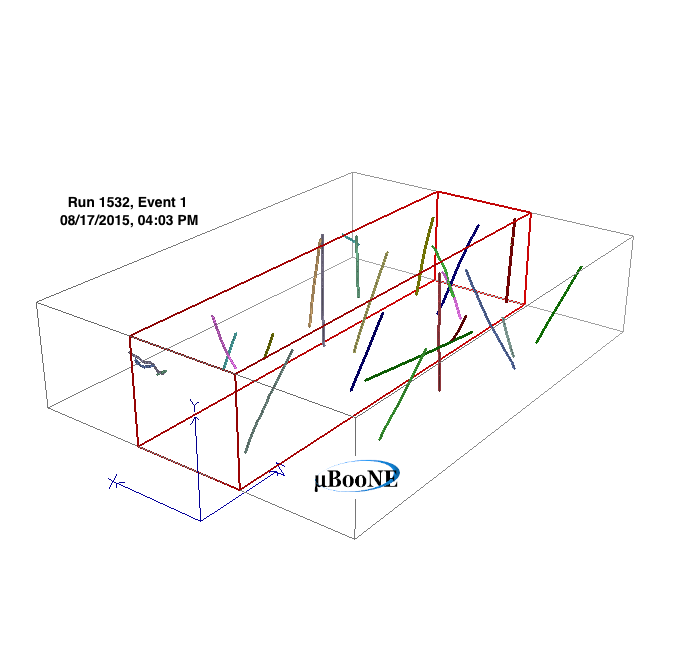
\includegraphics[width=0.9\textwidth]{Figures/UB_publicplot_3dcosmics.png}\\
\caption{\textit{A 3D event display showing measured cosmic tracks entering the MicroBooNE detector. The three boxes show the full readout window fo the detector which corresponds to 4.8 $ms$. The red highlighted box shows the physical volume of the TPC. The colored lines are 3D reconstructed cosmic tracks. Data taken in August, 2015.}}
\label{UB_publicplot_3dcosmics}
\end{figure}


Cosmic MID topologies include but are not limited to showers that radiate off of cosmic ray muons, and showers born from cosmic neutron scatters. The vast majority of MIDs from cosmics can be removed by requiring the reconstructed neutrino interaction is matched to a flash inside of the beam gate window. Given the ratio of beam gate window size to readout window size ($\frac{1.6\mu s}{4.8ms}=0.0003$), this requirement mitigates almost all of the cosmic backgrounds. However, the majority of triggered beam events are not triggered by a neutrino interaction in them but are instead triggered by a cosmic ray that arrived during the beam gate window. These events are referred to as ``in-time'' cosmics. Given the number of readouts triggered by cosmics inside of the beam gate window rather than neutrinos arriving inside of the beam gate window, the cosmics background can be sizable, especially in the relevant low energy region. The measured relative rate of reconstructed flash times inside the 1.6 $\mu s$ beam spill window with respect to the constant cosmic background in MicroBooNE is shown in Figure \ref{BNB_flashtime_data_plot}. The ratio of cosmic-triggered events to neutrino triggered events from that plot is 1 : 0.45, and only about half of those neutrino interactions are inside of the active volume (and are reconstructible), making the ratio closer to 5 triggered cosmic readouts for every neutrino triggered readout in which the neutrino is reconstructible.\\% It should be noted that a proper handling of these ``in-time'' cosmics will take into account events in which a cosmic flash inside of the beam gate window triggers a readout, and a reconstructed $\nu_e$ MID associated with a \textit{different} cosmic in the event gets incorrectly matched to the flash inside of the beam gate window.\\


\begin{figure}[ht!]
\centering
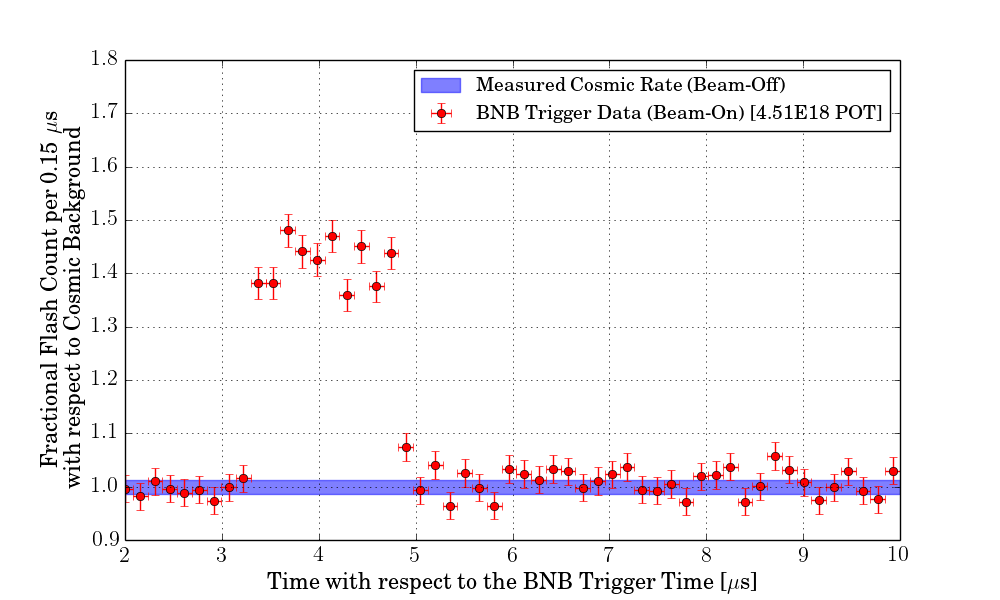
\includegraphics[width=0.9\textwidth]{Figures/BNB_flashtimeplot.png}\\
\caption{\textit{The measured distribution of flash times (requiring flashes greater than 50PE) with respect to the trigger time for BNB-triggered events, shown as a ratio to the expected cosmic rate from off-beam data. The blue band denoting the cosmic rate was centered at one, with a width corresponding to the measured uncertainty in the cosmic rate. A clear excess can be seen due to neutrinos between 3 and 5 $\mu$s after the trigger. This is where the neutrinos were expected based on the RWM signal arrival time. A total of 1.92E6 BNB triggered events (unbiased trigger) were used to produce this plot.}}
\label{BNB_flashtime_data_plot}
\end{figure}


In addition to these ``in-time'' cosmics (those that triggered a readout and arrived during the beam gate window), an additional cosmic background comes from events in which a \textit{neutrino} interacts inside of the beam gate window, triggering a readout, but an out-of-time cosmic MID gets incorrectly matched to the neutrino flash. These cosmic MIDs are appropriately referred to as ``out-of-time'' cosmics. The ``out-of-time" cosmic background is not included in this analysis, but its size relative to the ``in-time'' cosmics is small.\\

\subsection{Background Normalization}\label{LEE_background_normalization_section}
% Mention the beam induced backgrounds are normalized to POT, the cosmic backgrounds come from the open cosmic sample and are normalized to beam gate open time (which is assuming perfect flash matching).
As described in Section \ref{LEE_simulated_background_samples_section}, the simulated background samples used in this analysis can be classified either as beam-induced, or cosmic. Each beam-induced background has an associated simulated POT generated, and they are each normalized to $6.6\times10^{20}$ POT, the nominal amount of beam scheduled to be delivered to MicroBooNE over the course of three years running. The cosmic simulated sample does not have an associated POT, but instead has an associated total exposure time. The normalization of this sample must involve disregarding the event selection cut in which a reconstructed optical flash occurs within the timing of the beam gate window. The total beam-gate-open exposure time corresponding to $6.6\times10^{20}$ POT is 211 seconds:
\begin{equation}
\frac{6.6\times10^{20} POT}{5 \times 10^{12} \frac{POT}{spill}} \times 1.6\frac{\mu s}{spill} = 211 \text{ seconds}
\end{equation}
Therefore, a simple scale factor is computed based on the simulated cosmic exposure time.% Note that treatment of the cosmic background in this way is assuming that the reconstructed neutrino interaction in the TPC has been correctly flash-matched.


\subsection{Analysis Cuts and Results}\label{analysis_cut_descript_section}

%Description of the final cuts that are placed on the backgrounds (for example requiring the electron deposits more than 60 MeV of energy to mitigate michels, also requiring no pions in order to best mimic the MiniBooNE cuts). Showing the stacked backgrounds.

A number of additional analysis cuts are placed on the selected candidate $\nu_e^{CC}$ events. The purpose of these cuts is to first down-sample the selected $\nu_e^{CC}$ selected events into a sample of $\nu_e^{CCQE}$ events by removing those reconstructed as having pions in the final state. An additional reason to place these cuts is to mitigate backgrounds that the event selection algorithms were unable to remove themselves. The analysis cuts used are described here.\\

The analysis cuts placed are:
\begin{enumerate}
\item The reconstructed $\nu_e$ interaction is matched to a flash inside of the beam gate window (this cut is not placed on the cosmic background simulated sample for reasons described in Section \ref{LEE_background_normalization_section}).
\item If the reconstructed $\nu_e$ interaction has additional particles reconstructed to be in the final state, those particles are limited to protons only (using assumed perfect efficiency to tag a track as a proton). This down-samples the $\nu_e^{CC}$ selected sample to specifically $\nu_e^{CCQE}$.
\item Minimum primary $\nu_e^{CC}$ reconstructed electron energy deposited of 60 MeV.
\item A fiducial volume of 10 cm from all sides of the detector is placed on the neutrino interaction vertex.
\item A projected-backwards-distance-to-wall cut of 40 cm is placed on the primary $\nu_e^{CC}$ reconstructed electron.
\end{enumerate}
The projected-backwards-distance-to-wall cut is computed by back-projecting the reconstructed $\nu_e^{CC}$ electron along its shower axis until it intersects with the TPC boundaries. The distance between the electron start point and the wall intersection point is the distance on which the cut is placed.\\

%XXX  Mention ``what are the possible uncertainties that could make a significant change in the assumed backgrounds.''

The efficiency of the event selection algorithms with ``perfect reconstruction'' inputs to select signal events and to select background events (``MID efficiency'') is summarized in Table \ref{eventselection_efficiency_table}. The numerator of this efficiency is the number of events tagged as $\nu_e^{CCQE}$ candidate interactions and the denominator is the true number of events with the specified interaction type. The second column in the table does not include the additional final analysis selection cuts which are placed on the reconstruction interactions in the efficiency numerator, and the third column does. The background categories are described in more detail in Section \ref{LEEbackgroundtopologiessection}. In the case of the cosmic background category, the denominator is the true number of events triggered by a cosmic arriving within the beam gate window that do not include a neutrino interaction.\\


\begin{table}
\begin{tabular}{ |p{4cm}|p{3cm}|p{6cm}|  }
 \hline
 \multicolumn{3}{|c|}{Event Selection Efficiencies} \\
 \hline
 True Event Type & Efficiency & Efficiency Including Analysis Cuts \\
 \hline \hline
 $\nu_e^{CCQE}$ & 0.8209 & 0.6142\\\hline
 
 $\nu_\mu$CC & 0.0068 & 0.0002\\\hline

 $\nu_x$NC & 0.0086 & 0.0013\\\hline

 B.I.T.E. & 0.0107 & 0.0005 \\\hline

 Cosmic & 0.0588 & 0.0012\\\hline

 \hline
\end{tabular}
\caption{\textit{Event selection efficiencies on ``perfect reconstruction''.}}\label{eventselection_efficiency_table}
\end{table}



The backgrounds to the $\nu_e^{CCQE}$ appearance search in MicroBooNE are shown in Figure \ref{LEE_stackedbackgrounds_nosignal_withanalysiscuts_fig}, normalized to the nominal MicroBooNE expected POT. The event selection is described in Section \ref{LEE_eventselection_section}, the background topologies described in Section \ref{LEEbackgroundtopologiessection}, the relative normalization between samples described in Section \ref{LEE_background_normalization_section}, and the energy reconstruction described in Section \ref{LEE_EnergyReco_section}.


\begin{figure}[ht!]
\centering
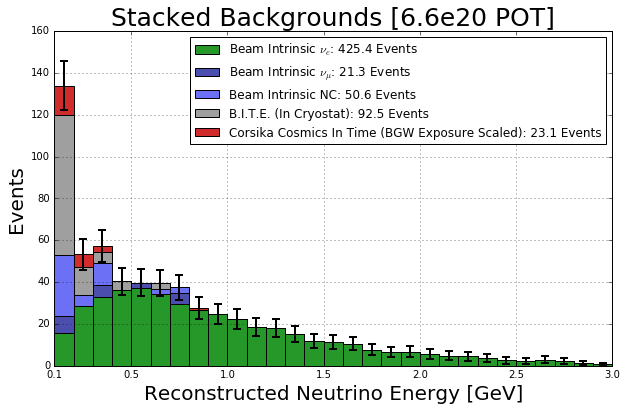
\includegraphics[width=0.9\textwidth]{Figures/LEE_stackedbackgrounds_nosignal_withAnalysisCuts.png}\\
\caption{\textit{The backgrounds to the $\nu_e^{CCQE}$ appearance search in MicroBooNE. The event selection is described in Section \ref{LEE_eventselection_section}, the background topologies described in Section \ref{LEEbackgroundtopologiessection}, the relative normalization between samples described in Section \ref{LEE_background_normalization_section}, and the energy reconstruction described in Section \ref{LEE_EnergyReco_section}.}}
\label{LEE_stackedbackgrounds_nosignal_withanalysiscuts_fig}
\end{figure}





\section{MiniBooNE Low Energy Excess Signal Modeling In MicroBooNE}\label{MBLEESignalModeling_section}
% Here is where I describe how I come up with my scaled signal shape and normalization. Simulated sample are intrinsic nues, since I'm assuming the excess is coming from beam nues. Shape comes from MiniBooNE published data (excess events evis distribution and uz distribution along with the CCQE formula). Normalization comes from size of MiniBooNE excess with respect to size of MiniBooNE intrinsic nue background in a specific region (excess should be larger than the intrinsic nue background in the low CCQE-energy region... this was Bill's recent suggestion). This section will probably be several pages long.
This section describes how the signal sample is generated for this sensitivity study, along with the necessary assumptions made in the process. First, the signal is assumed to originate from beam-induced $\nu_e^{CCQE}$ interactions (this is the electron-like hypothesis for the excess). No study for a photon-like excess is described in this thesis. In this electron-like excess search, the signal sample consists of simulated intrinsic $\nu_e^{CCQE}$ interactions from the BNB generated uniformly throughout the MicroBooNE TPC. The energy and angle of these events are re-weighted to match the published energy and angle distributions of the excess as observed by MiniBooNE. \\

The MiniBooNE public data set \cite{MB_lee_datarelease} provides one dimensional distributions of $u_z$, $E_{vis}$, and $E_\nu^{CCQE}$ for the excess events, where $u_z$ is the z-direction cosine (the z- component of the unit momentum) of the observed particle in the low energy excess sample, $E_{vis}$ is the visible energy associated with the event, and $E_{\nu}^{CCQE}$ is the calculated neutrino energy assuming the interaction was charged current quasi-elastic (see Equation (\ref{MB_CCQE_formula})).\\

Given these three one-dimensional distributions, a two-dimensional distribution of $u_z$ vs. $E_{vis}$ is built by using the CCQE formula here that as shown in Equation (\ref{MB_CCQE_formula})\footnote{The careful reader will note that the CCQE energy formula should use lepton energy, $E_e$, but here $E_{vis}$ is used instead. This is assuming that the lepton energy is the same as the visible energy.}. By comparing the MicroBooNE signal sample two-dimensional histogram of $\nu_e^{CCQE}$ electron $u_z$ vs. $E_{vis}$ to this MiniBooNE excess distribution, re-weighting factors are computed to reshape the MicroBooNE signal sample to match the MiniBooNE excess in this parameter space.\\

The strategy to generate the MiniBooNE excess two dimensional distribution is as follows:
\begin{enumerate}
\item Draw independently from each of the the two one-dimensional histograms: $u_z$ and $E_{vis}$.
\item For every drawn pair, calculate the corresponding $E_\nu^{CCQE}$ with Equation \ref{MB_CCQE_formula} and decide whether to accept it according to the published MiniBooNE excess $E_\nu^{CCQE}$ one-dimensional distribution.
	\begin{itemize}
	\item The probably of accepting a calculated $E_\nu^{CCQE}$ that falls within the bin's boundaries is equal to the height of the unit-normalized $E_\nu^{CCQE}$ distribution in any given bin.
	\end{itemize}
\item Repeat this process until the number of accepted pairs = N $\times$ Integrated number of excess events in the $u_z$ distribution (choosing N to be large: E.G. N = 1000). This two dimensional distribution represents the observed excess as seen from MiniBooNE.
\item Divide this distribution by the MiniBooNE published efficiency for single electrons (given as a function of $E_{vis}$) to uncover the shape of the true excess event distribution in MiniBooNE\footnote{No efficiency as a function of any other variable (E.G. $u_z$) has been published by MiniBooNE.}.
\item Smooth the resulting two-dimensional distribution with a default ROOT TH2::Smooth() function.
\end{enumerate}
The resulting two-dimensional distribution of $u_z$ vs. $E_{vis}$ for the true MiniBooNE excess events is shown in Figure \ref{MBth2dfig}.


\begin{figure}[ht!]
\centering
	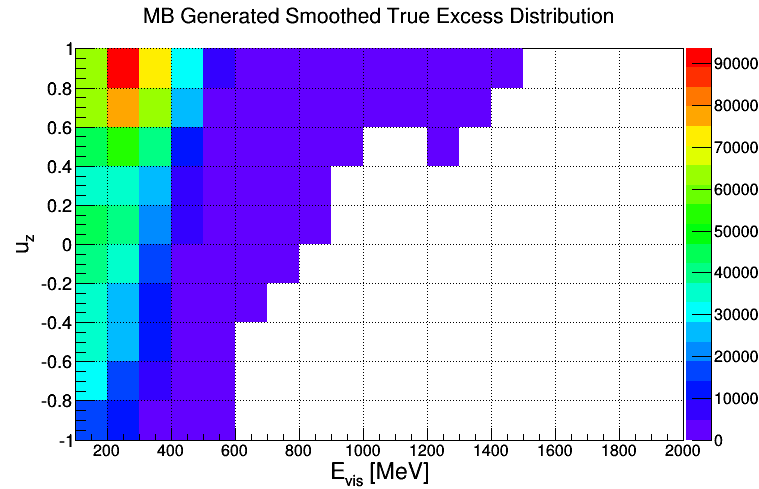
\includegraphics[width=0.9\textwidth]{Figures/miniboone_excess_th2d.png} \\
\caption{\textit{The computed distribution of $u_z$ (how forward-going the event is) vs. $E_{vis}$ for N = 1000 times the MiniBooNE low energy excess (raw) events.}}\label{MBth2dfig}
\end{figure}

While the shape of the simulated MicroBooNE signal events is determined by the above process, the absolute normalization of this sample is computed by comparing the relative size of the signal with respect to the intrinsic $\nu_e$ backgrounds as observed by MiniBooNE. This is appropriate to do only because of the assumption that the origin of the low energy excess is intrinsic BNB $\nu_e$s. From MiniBooNE data and MC, there are 187.7 excess signal events and 148.4 intrinsic $\nu_e$ events in the $E_\nu^{CCQE}$ energy range from 100 to 600 MeV. In this analysis, the number of intrinsic $\nu_e$ events in that $E_\nu^{CCQE}$ energy range in MicroBooNE is computed to be 159.8, and therefore the simulated signal sample is normalized to have 159.8*(187.7/148.4)=201.3 events in that $E_\nu^{CCQE}$ energy range.\\





















\subsection{Sensitivity Results}

Shown in Figure \ref{LEE_perfectreco_fullstack_fig} is the previously shown stacked backgrounds with the scaled MiniBooNe low energy excess signal included. Also labeled on the plot is the computed significance of 11.57$\sigma$, including only statistical errors. The details on the computation of the significance is described in the next section.

\begin{figure}[ht!]
\centering
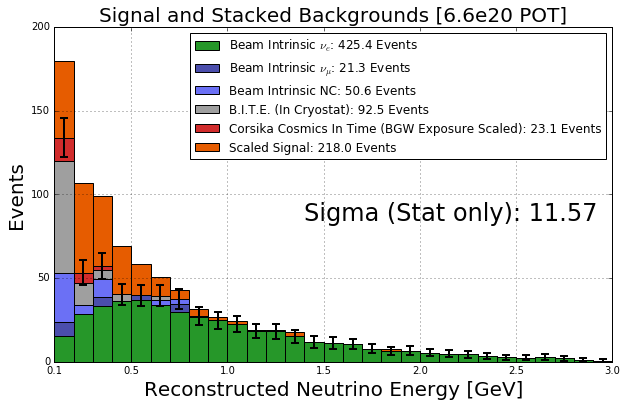
\includegraphics[width=0.9\textwidth]{Figures/LEE_perfectreco_fullstack_WithAnalysisCuts.png}\\
\caption{\textit{The backgrounds to the $\nu_e^{CCQE}$ appearance search in MicroBooNE with scaled signal drawn. The event selection is described in Section \ref{LEE_eventselection_section}, the background topologies described in Section \ref{LEEbackgroundtopologiessection}, the relative normalization between samples described in Section \ref{LEE_background_normalization_section}, and the energy reconstruction described in Section \ref{LEE_EnergyReco_section}. The scaled signal is described in Section \ref{MBLEESignalModeling_section}.}}
\label{LEE_perfectreco_fullstack_fig}
\end{figure}

% Here I show the stacked background with the scaled signal on top, I describe how I compute a sensitivity (statistical errors only for now... I could do a back-of-the-envelope estimate of systematic errors which are dominated by flux). ``Probably do need some estimates of systematic uncertainties. Also will you say anything about an electron LEE vs a photon LEE sensitivity''.
\subsubsection{Significance Calculation}
For a given stacked background plot with a scaled signal on top, the statistical-only significance is can be computed as:
\begin{equation}\label{chisquaresigeqtn}
\sigma = \sqrt{\Delta \chi^2} = \sqrt{\vec{S}^TE^{-1}\vec{S}}
\end{equation}
where $\vec{S}$ is a vector containing the size of the signal, with length equal to the number of bins in the histogram, $n$, and $E$ is the $n\times n$ statistical-only covariance matrix (diagonal matrix with entries equal to the summed number of background events per bin).


\subsubsection{Results with Realistic Shower Reconstruction Efficiency}
So far in this analysis, the shower reconstruction efficiency has been 100\% because the input objects are ``perfect reconstruction''. In order to emulate a more realistic potential shower reconstruction efficiency, an additional study has been done in which the shower reconstruction efficiency is modeled in an energy dependent way, with a maximum of 85\% efficiency for showers with energy included in this analysis (above 60 MeV deposited). The value of 85\% was chosen because this is approximately the maximum shower efficiency published by the ICARUS collaboration \cite{ICARUS_showereff_source}. The resulting stacked background histogram with modeled signal is shown in Figure \ref{LEE_recoemu_fullstack_fig}. The computed (statistical only) significance when realistic shower reconstruction efficiencies are included in the analysis is 10.10$\sigma$.


\begin{figure}[ht!]
\centering
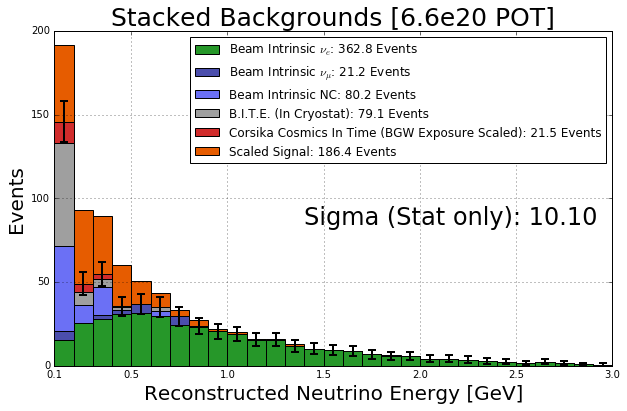
\includegraphics[width=0.9\textwidth]{Figures/LEE_recoemu_fullstack_WithAnalysisCuts.png}\\
\caption{\textit{The backgrounds to the $\nu_e^{CCQE}$ appearance search in MicroBooNE with scaled signal drawn. The event selection is described in Section \ref{LEE_eventselection_section}, the background topologies described in Section \ref{LEEbackgroundtopologiessection}, the relative normalization between samples described in Section \ref{LEE_background_normalization_section}, and the energy reconstruction described in Section \ref{LEE_EnergyReco_section}. The scaled signal is described in Section \ref{MBLEESignalModeling_section}. Here the shower reconstrution efficiency has been decreased from the ``perfect reconstruction'' value of 100\% to 85\% to emulate possible realistic shower reconstruction efficiencies.}}
\label{LEE_recoemu_fullstack_fig}
\end{figure}

Note that in comparing Figure \ref{LEE_perfectreco_fullstack_fig} to Figure \ref{LEE_recoemu_fullstack_fig}, not all sample sizes are simply reduced by 15\%. For example, the intrinsic NC backgrounds actually increase when the shower reconstruction efficiency is decreased. This is because these backgrounds arise primarily from $\pi^0$ decays, and they are mitigated by event selection algorithms that locate both subsequent photon showers pointing back to a common origin and correlate them together. With reduced shower reconstruction efficiency, sometimes only one of the $\pi^0$ decay showers gets reconstructed and subsequently gets misidentified as a candidate $\nu_e^{CC}$ electron.

\subsubsection{Systematic Error Estimates}

In order to compute a realistic significance to the low energy excess in this analysis, a treatment of systematic uncertainties is necessary. While this is a detailed and important study, a conservative simplified estimation of these uncertainties is described here.\\

Previous studies described in the proposal for the Short Baseline Neutrino experiment (which includes MicroBooNE as one of three detectors) \cite{SBNproposal} quote the integrated $\nu_e$ and $\nu_\mu$ flux uncertainties to be on the order of 10 to 15\%. This number comes from systematic uncertainty estimates related to primary production of $\pi^+$, $\pi^-$, $K^+$, $K^-$, and $K^0_L$ in $p+Be$ collisions at 8 GeV in the BNB, secondary interactions of $p$, $n$, $\pi^\pm$ in the beryllium target and aluminum horn, and beam focusing with the magnetic horn.\\

The SBN studies also quote the cross section uncertainties to be on the order of 20\%. This number comes from varying model parameters in the GENIE neutrino interaction generator to determine 1$\sigma$ uncertainties. Parameters varied include axial mass for CCQE events, axial mass for CC resonant neutrino production, axial mass for NC resonant production, neutral current normalization, and switching of deep inelastic scattering nuclear models. A full list of parameters varied and their 1$\sigma$ uncertainties can be found in the GENIE manual, Section 8.1 \cite{GENIEsource}.\\

While many of these uncertainties are strongly correlated across energy bins, a very conservative approach is to simply include a flat, uncorrelated flux uncertainty of 15\% and a similarly flat, uncorrelated cross section uncertainty of 20\%. These uncertainties are applied to all beam-induced backgrounds in this analysis. The systematic uncertainties on the cosmic-induced backgrounds are not known, but given the relatively small size of these backgrounds in this analysis, even a systematic of 50\% would have small impact on the final computed significance, so this systematic is neglected. Additional uncertainties from sources including detector systematics are expected to be sub-dominant to the relatively large flux and cross-section systematics, and are therefore similarly neglected. It is important to note that these conservative estimates are ignoring many \textit{in situ} measurements that can be done in MicroBooNE to constrain the uncertainties, as MiniBooNE did. For example, a parallel $\nu_\mu^{CC}$ analysis can constrain much of the $\nu_e$ flux uncertainties. Also, NC $\pi^0$ measurements help constrain cross section $\times$ flux uncertainties for that process.\\

In order to include the flux and cross-section systematics in the significance calculation, Equation \ref{chisquaresigeqtn} is modified. As quoted, $E$ is the $n\times n$ diagonal covariance matrix with entries equal to the summed number of background events per bin. To include the flux and cross-section systematics, $E$ is modified as
\begin{equation}\label{LEE_emtx_systematics}
E = E_{\text{stat}} + E_{\text{flux}} + E_{\text{xsec}}
\end{equation}
where $E_{\text{stat}}$ is the previous statistical-only covariance matrix, while $E_{\text{flux}}$ represents the assumed uncorrelated flux systematic and $E_{\text{xsec}}$ the assumed uncorrelated cross section systematic. $E_{\text{flux}}$ is diagonal with entries equal to the number of beam-induced (non-cosmic) background events in that bin times the fractional uncertainty, squared:
\begin{equation}\label{LEE_flux_emtx}
E_{\text{flux}}^{i,i} = (N_{\text{beam-induced}}^i*0.15)^2
\end{equation}
and $E_{\text{xsec}}$ is similarly diagonal:
\begin{equation}\label{LEE_xsec_emtx}
E_{\text{xsec}}^{i,i} = (N_{\text{beam-induced}}^i*0.20)^2
\end{equation}

With these systematic uncertainties included in the significance calculation, with realistic shower reconstruction efficiencies included the significance is reduced from 10.10$\sigma$ (statistical only) to 6.52$\sigma$. Note that assuming these systematics are uncorrelated is very conservative. A complete summary of MicroBooNE's computed significance to the MiniBooNE low energy excess assuming an electron-like signal hypothesis for ``perfect reconstructed'' objects, ``perfect reconstructed objects'' with simulated realistic shower reconstruction efficiency, with and without conservative systematic uncertainties can be found in Table \ref{LEE_final_significance_table}.


\begin{table}
\begin{tabular}{ |p{5cm}|p{5cm}|p{5cm}|  }
 \hline
 \multicolumn{3}{|c|}{MicroBooNE Sensitivity Significances} \\
 \hline
 ``Perfect Reco'' (stat only) & ``Realistic Reco'' (stat only) & ``Realistic Reco'' (stat+sys) \\
 \hline \hline
 11.57$\sigma$ & 10.10$\sigma$ & 6.52$\sigma$\\\hline
 
 \hline
\end{tabular}
\caption{\textit{Summary of computed significances to the MiniBooNE low energy excess in MicroBooNE assuming an electron-like signal hypothesis.}}\label{LEE_final_significance_table}
\end{table}



\subsubsection{Next Steps}
The described ``perfect reconstruction'' sensitivity study to an electron-like excess is an important tool for MicroBooNE. The event selection algorithms have been developed with these objects, and are ready to be used out-of-the-box when automated track and shower reconstruction efforts become more fruitful in the future. Additionally, this sensitivity study can be used to set goals for the experiment by smearing or modifying the ``perfect reconstruction'' objects. For example, with this analysis the sensitivity to the low energy excess can be computed as a function of shower reconstruction efficiency to drive the effort to reach 5$\sigma$. Also, the sensitivity as a function of POT delivered has already been used to guide discussions on data blinding, for example to address how much can remain unblinded for reconstruction development without biasing the $\nu_e$ search.\\

As mentioned, no photon-like excess search is described in this thesis. It is important to determine a sensitivity to an electron-like excess as well as a photon-like excess, because the true origin of the excess is still unknown. In order to conduct a photon-like excess search, event selection algorithms and analysis cuts would have to be developed to search for single photon events rather than single electron events.\\

An important takeaway from this electron-like excess analysis is that systematics play an important role in the ultimate sensitivity. The flux systematic is particularly large. As shown, the largest background in the MicroBooNE low energy excess search is from intrinsic $\nu_e$s in the beam, which come from either muon decay in the beam-line, or kaon decay in the beam-line. In the low energy region, the majority of intrinsic $\nu_e$s come from muon decay, which is tied to the observed $\nu_\mu$ events, as demonstrated by MiniBooNE. Constraining the remaining $\nu_e$s from kaon decay can be done by observing the high energy $\nu_\mu$ rate, the topic of the next chapter.

